
\documentclass[a4paper, 12pt, hidelinks]{book}

\usepackage[utf8x]{inputenc}   % omogoča uporabo slovenskih črk v UTF-8
\PrerenderUnicode{č}
\PrerenderUnicode{š}
\PrerenderUnicode{ž}

\usepackage[titletoc,page]{appendix}

\usepackage[slovene,english]{babel}  % slovenski delilni vzorci ipd.
\usepackage[pdftex]{graphicx}  % omogoča vlaganje slik različnih formatov
\usepackage{fancyhdr}          % poskrbi, na primer, za glave strani
\usepackage{amssymb}           % dodatni simboli
\usepackage{amsmath}
\usepackage{fixltx2e}          % textsubscript etc. (XXX: used anywhere here?)
\usepackage{color}
\usepackage{array}
\usepackage{tabulary}
\usepackage{icomma}            % comma as a decimal separator

\usepackage{pgfplots}

\usepackage{numprint}          % number formating
\npthousandsep{.}\npthousandthpartsep{}\npdecimalsign{,}

\usepackage[lined,plain,linesnumbered]{algorithm2e}
\usepackage{setspace}

\setlength{\headheight}{29.5pt}

% translate appendices' titles
\addto\captionsslovene{%
  \renewcommand\appendixpagename{Priloge}
  \renewcommand\appendixname{Priloga}
}

% remove page number from appendices title page
\let\plainappendixpage\appendixpage
\makeatletter
\renewcommand{\appendixpage}{%
  \begingroup
  \let\ps@plain\ps@empty
  \plainappendixpage
  \endgroup}
\makeatother

% swap page margins (inner margins should be bigger - for binding purposes)
\let\tmp\oddsidemargin
\let\oddsidemargin\evensidemargin
\let\evensidemargin\tmp
\reversemarginpar

% reduce line spacing for algorithms to save space
\usepackage{etoolbox}
\AtBeginEnvironment{algorithm}{\setstretch{1.05}\small}

\raggedbottom  % fixes some unwanted vertical gaps

% change algorithm label name
\renewcommand{\algorithmcfname}{Psevdokoda}


\renewcommand*{\familydefault}{\rmdefault}  % default font family (roman)
\renewcommand{\baselinestretch}{1.3}  % ustrezen razmik med vrsticami

\renewcommand{\arraystretch}{1.3}  % razmik med vrsticami tabel
\AtBeginEnvironment{tabular}{\small}

%oznake strani
\renewcommand{\chaptermark}[1]%
{\markboth{\MakeUppercase{\thechapter.\ #1}}{}}
\renewcommand{\sectionmark}[1]%
{\markright{\MakeUppercase{\thesection.\ #1}}}
\renewcommand{\headrulewidth}{0.5pt} \renewcommand{\footrulewidth}{0pt}
\fancyhf{}
\fancyhead[LE,RO]{\sl \thepage} \fancyhead[LO]{\sl \rightmark}
\fancyhead[RE]{\sl \leftmark}

\newcommand{\BibTeX}{{\sc Bib}\TeX}

\newcommand{\autfont}{\Large}
\newcommand{\titfont}{\LARGE\bf}
\newcommand{\newterm}{\textit}

\newcommand{\TODO}[1]{\textcolor{red}{(TODO: #1)}}
\newcommand{\sub}{\textsubscript}

\newcommand{\clearemptydoublepage}{
	\newpage{\pagestyle{empty}\cleardoublepage}}
\setcounter{tocdepth}{2}	      % globina kazala

% konstrukti
\newtheorem{izrek}{Izrek}[chapter]

%\newtheorem{trditev}{Trditev}[izrek]
\newenvironment{dokaz}{\emph{Dokaz.}\ }{\hspace{\fill}{$\Box$}}

\newenvironment{itquote}
{\begin{quote}\itshape}
{\end{quote}}


\usepackage[pdftex, colorlinks=true,
						citecolor=black, filecolor=black,
						linkcolor=black, urlcolor=black,
						pagebackref=false,
						pdfproducer={LaTeX}, pdfcreator={LaTeX}]{hyperref}


%%%%%%%%%%%%%%%%%%%%%%%%%%%%%%%%%%%%%%%%
%	DIPLOMA INFO
%%%%%%%%%%%%%%%%%%%%%%%%%%%%%%%%%%%%%%%%
\newcommand{\ttitle}{Primerjava dveh strategij dinamične replikacije}
\newcommand{\ttitleEn}{Comparison of two dynamic data replication strategies}
\newcommand{\tsubject}{\ttitle}
\newcommand{\tsubjectEn}{\ttitleEn}
\newcommand{\tauthor}{Peter Lamut}
\newcommand{\tkeywords}{
podatkovno omrežje, dinamična replikacija, Fast Spread, odzivni čas,
porabljena pasovna širina, diskretna simulacija
}
\newcommand{\tkeywordsEn}{
data grid, dynamic replication, Fast Spread, response time, bandwidth used,
discrete event simulation
}



\usepackage{hyperref}
%%%%%%%%%%%%%%%%%%%%%%%%%%%%%%%%%%%%%%%%
%	HYPERREF SETUP
%%%%%%%%%%%%%%%%%%%%%%%%%%%%%%%%%%%%%%%%
\hypersetup{pdftitle={\ttitle}}
\hypersetup{pdfsubject=\ttitleEn}
\hypersetup{pdfauthor={\tauthor, jeti51@gmail.com}}
\hypersetup{pdfkeywords=\tkeywordsEn}


%%%%%%%%%%%%%%%%%%%%%%%%%%%%%%%%%%%%%%%%%%%%%%%%%%%%%%%%%%%%%%%%%%%%%%%%%%%%%%%
%% PDF-A
%%%%%%%%%%%%%%%%%%%%%%%%%%%%%%%%%%%%%%%%%%%%%%%%%%%%%%%%%%%%%%%%%%%%%%%%%%%%%%%

%%%%%%%%%%%%%%%%%%%%%%%%%%%%%%%%%%%%%%%%
% define medatata
%%%%%%%%%%%%%%%%%%%%%%%%%%%%%%%%%%%%%%%%
\def\Title{\ttitle}
\def\Author{\tauthor, jeti51@gmail.com}
\def\Subject{\ttitleEn}
\def\Keywords{\tkeywordsEn}

%%%%%%%%%%%%%%%%%%%%%%%%%%%%%%%%%%%%%%%%
% \convertDate converts D:20080419103507+02'00' to 2008-04-19T10:35:07+02:00
%%%%%%%%%%%%%%%%%%%%%%%%%%%%%%%%%%%%%%%%
\def\convertDate{%
    \getYear
}

{\catcode`\D=12
 \gdef\getYear D:#1#2#3#4{\edef\xYear{#1#2#3#4}\getMonth}
}
\def\getMonth#1#2{\edef\xMonth{#1#2}\getDay}
\def\getDay#1#2{\edef\xDay{#1#2}\getHour}
\def\getHour#1#2{\edef\xHour{#1#2}\getMin}
\def\getMin#1#2{\edef\xMin{#1#2}\getSec}
\def\getSec#1#2{\edef\xSec{#1#2}\getTZh}
\def\getTZh +#1#2{\edef\xTZh{#1#2}\getTZm}
\def\getTZm '#1#2'{%
    \edef\xTZm{#1#2}%
    \edef\convDate{\xYear-\xMonth-\xDay T\xHour:\xMin:\xSec+\xTZh:\xTZm}%
}

\expandafter\convertDate\pdfcreationdate

%%%%%%%%%%%%%%%%%%%%%%%%%%%%%%%%%%%%%%%%
% get pdftex version string
%%%%%%%%%%%%%%%%%%%%%%%%%%%%%%%%%%%%%%%%
\newcount\countA
\countA=\pdftexversion
\advance \countA by -100
\def\pdftexVersionStr{pdfTeX-1.\the\countA.\pdftexrevision}


%%%%%%%%%%%%%%%%%%%%%%%%%%%%%%%%%%%%%%%%
% XMP data
%%%%%%%%%%%%%%%%%%%%%%%%%%%%%%%%%%%%%%%%
\usepackage{xmpincl}
\includexmp{pdfa-1b}

%%%%%%%%%%%%%%%%%%%%%%%%%%%%%%%%%%%%%%%%
% pdfInfo
%%%%%%%%%%%%%%%%%%%%%%%%%%%%%%%%%%%%%%%%
\pdfinfo{%
    /Title    (\ttitle)
    /Author   (\tauthor, jeti51@gmail.com)
    /Subject  (\ttitleEn)
    /Keywords (\tkeywordsEn)
    /ModDate  (\pdfcreationdate)
    /Trapped  /False
}


%%%%%%%%%%%%%%%%%%%%%%%%%%%%%%%%%%%%%%%%%%%%%%%%%%%%%%%%%%%%%%%%%%%%%%%%%%%%%%%
%%%%%%%%%%%%%%%%%%%%%%%%%%%%%%%%%%%%%%%%%%%%%%%%%%%%%%%%%%%%%%%%%%%%%%%%%%%%%%%




\begin{document}
\selectlanguage{slovene}
\frontmatter
\setcounter{page}{1} %
\renewcommand{\thepage}{}  % preprecimo težave s številkami strani v kazalu


%%%%%%%%%%%%%%%%%%%%%%%%%%%%%%%%%%%%%%%%
%platnica
\label{platnica}
\thispagestyle{empty}%
\begin{center}
    {\large\sc Univerza v Ljubljani\\%
      Fakulteta za računalništvo in informatiko}%
    \vskip 10em%
    {\autfont Peter Lamut\par}%
    {\titfont Primerjava dveh strategij dinamične replikacije \par}%
    {\vskip 2em \textsc{DIPLOMSKO DELO NA UNIVERZITETNEM ŠTUDIJU
    RAČUNALNIŠTVA IN INFORMATIKE}\par}%
    \vfill\null%

    {\vskip 2em \large Ljubljana, 2014 \par}%
\end{center}

% prazna stran
\clearemptydoublepage

%%%%%%%%%%%%%%%%%%%%%%%%%%%%%%%%%%%%%%%%
%naslovnica (enaka kot platnica, le da še z navedbo mentorja
\label{naslovnica}
\thispagestyle{empty}%
\begin{center}
    {\large\sc Univerza v Ljubljani\\%
      Fakulteta za računalništvo in informatiko}%
    \vskip 10em%
    {\autfont Peter Lamut\par}%
    {\titfont Primerjava dveh strategij dinamične replikacije \par}%
    {\vskip 2em \textsc{DIPLOMSKO DELO NA UNIVERZITETNEM ŠTUDIJU
    RAČUNALNIŠTVA IN INFORMATIKE}\par}%
    \vfill\null%
    {\large \textsc{Mentor}: doc.\ dr.\ Boštjan Slivnik\par}%
    {\vskip 2em \large Ljubljana, 2014 \par}%
\end{center}

% prazna stran
\clearemptydoublepage


%%%%%%%%%%%%%%%%%%%%%%%%%%%%%%%%%%%%%%%%
%copyright stran
\label{copyright_page}
\thispagestyle{empty}
\vspace*{8cm}

{\small \noindent
Rezultati diplomskega dela so intelektualna lastnina avtorja in Fakultete za
ra\-ču\-nal\-niš\-tvo in informatiko Univerze v Ljubljani.
Za objavljanje ali izkoriščanje rezultatov di\-plom\-ske\-ga dela je potrebno
pisno soglasje avtorja, Fakultete za ra\-ču\-nal\-niš\-tvo in
informatiko ter mentorja.}%

\begin{center} 
\mbox{}\vfill
\emph{Besedilo je oblikovano z urejevalnikom besedil \LaTeX.} 
\end{center}


% prazna stran
\clearemptydoublepage


%%%%%%%%%%%%%%%%%%%%%%%%%%%%%%%%%%%%%%%%
% izjava o avtorstvu
\label{izjava_avtorstvo}

\vspace*{1cm}
\begin{center} 
{\Large \textbf{\sc Izjava o avtorstvu diplomskega dela}}
\end{center}

\vspace{1cm}
\noindent Spodaj podpisani Peter Lamut,
z vpisno številko \textbf{63000200}, sem avtor diplomskega dela z naslovom:
   
\vspace{0.5cm}
\centerline{\emph{Primerjava dveh strategij dinamične replikacije}}

\vspace{1.5cm}
\noindent S svojim podpisom zagotavljam, da:

\begin{itemize}
	\item sem diplomsko delo izdelal samostojno pod mentorstvom doc.\ dr.\ 
	Boštjana Slivnika,

	\item so elektronska oblika diplomskega dela, naslov (slov., angl.),
	 povzetek (slov., angl.) ter ključne besede (slov., angl.) identični
	 s tiskano obliko diplomskega dela,
	
	\item soglašam z javno objavo elektronske oblike diplomskega dela
	v zbirki ``Dela FRI''.
\end{itemize}

\vspace{1cm}

\noindent V Ljubljani, dne 27. junija 2014 \hfill
Podpis avtorja:

% prazna stran
\clearemptydoublepage


%%%%%%%%%%%%%%%%%%%%%%%%%%%%%%%%%%%%%%%%
% zahvala

\label{zahvala}
\thispagestyle{empty}\mbox{}\vfill\null\it%
Rad bi se zahvalil mentorju doc.~dr.~Boštjanu Slivniku za vse koristne nasvete
in usmerjanje pri izdelavi diplomskega dela.

Zahvaljujem se teti Veri, ki je diplomsko delo lektorirala in povzetek
prevedla v angleški jezik.

Prav tako se zahvaljujem svoji dragi Janji za vso moralno podporo med pisanjem
diplome.

Na koncu pa bi se rad zahvalil tudi prijateljema Darku Mariču in Anžetu
Šuštarju, ki pri izdelavi diplomskega dela sicer nista pomagala popolnoma nič,
se jima je pa zdelo zabavno, da bi bila kljub temu omenjena. ;-)

\vskip 1.5em

\noindent
(Peter Lamut, junij 2014)

\rm\normalfont

% prazna stran
\clearemptydoublepage


%%%%%%%%%%%%%%%%%%%%%%%%%%%%%%%%%%%%%%%%
% kazalo
\label{kazalo}
\def\thepage{}% preprecimo tezave s stevilkami strani v kazalu 
\tableofcontents{}


% prazna stran
\clearemptydoublepage


%%%%%%%%%%%%%%%%%%%%%%%%%%%%%%%%%%%%%%%%
% povzetek
\addcontentsline{toc}{chapter}{Povzetek}
\chapter*{Povzetek}

Podatkovno omrežje je množica med seboj povezanih računalnikov na raz\-ličnih
geografskih lokacijah, katerega cilj je razpoložljivost podatkov in odpor\-nost
na napake. Z izbiro ustrezne replikacijske strategije želimo doseči takšno
razporeditev datotek v omrežju, da je njegovo delovanje čim boljše (z
\mbox{vidika} odzivnih časov in porabljene pasovne širine). V diplomskem delu
sta obravnavana dva znanstvena članka istih avtorjev, v katerih predlagajo
izboljšave dinamične replikacijske strategije \textit{Fast Spread},
vendar pa njihovih rezultatov ni bilo možno ponoviti. Poleg tega se je zaradi
velike medsebojne podobnosti člankov pojavil tudi resen sum recikliranja
le-teh.\ Diplomsko delo v uvodu najprej predstavi podatkovna omrežja s
teoretičnega vidika, nato opiše, kako je potekalo testiranje v člankih
predlaganih strategij, v nadaljevanju pa potem podrobno obravnava vse
ugotovljene pomanjkljivosti člankov, vključno z njuno (pre)veliko podobnostjo.

\section*{Ključne besede}
podatkovno omrežje, dinamična replikacija, Fast Spread, odzivni čas,
porabljena pasovna širina, diskretna simulacija


% prazna stran
\clearemptydoublepage


%%%%%%%%%%%%%%%%%%%%%%%%%%%%%%%%%%%%%%%%
% abstract
\selectlanguage{english}
\addcontentsline{toc}{chapter}{Abstract}
\chapter*{Abstract}

A data grid is a set of mutually connected computers at geographically
different sites, whose aim is to achieve a good availability of the data
and a resistance to errors. By choosing an adequate replication strategy one
wants to achieve such an arrangement of the files in the grid that the
performance thereof is as good as possible (with regard to the response time
and to the bandwidth used). The diploma thesis deals with two scientific papers
of the same authors, wherein they suggest improvements of the dynamic
replication strategy Fast Spread, yet it has not been possible to repeat their
results. Additionally, the great similarity of the papers gives rise to a
strong suspicion of autoplagiarism. In the introduction of the diploma thesis,
data grids are presented from a theoretical point of view, then it is
described how the testing of the strategies suggested in the papers took place
and, subsequently, all established defects of the papers including their (too)
great similarity are dealt with.

\section*{Keywords}
data grid, dynamic replication, Fast Spread, response time, bandwidth used,
discrete event simulation

\selectlanguage{slovene}

% prazna stran
\clearemptydoublepage


%%%%%%%%%%%%%%%%%%%%%%%%%%%%%%%%%%%%%%%%
\mainmatter
\setcounter{page}{1}
\pagestyle{fancy}

\chapter{Uvod}

\section{Splošno o podatkovnih omrežjih}

Podatkovno omrežje (angl.~\textit{Data Grid}) je množica med seboj
povezanih ra\-ču\-nal\-ni\-kov na različnih geografskih lokacijah, ki
uporabnikom omogočajo nalaganje, hranjenje in medsebojno izmenjavanje datotek
\cite{dgrid_def}. Glavna cilja takšnega omrežja sta čim nižji odzivni čas na
zahtevke za podatke in odpornost na morebitne motnje v delovanju posameznih
vozlišč (visoka razpoložljivost) \cite{dgrid_def}.

\section{Replikacija podatkov}

Ko uporabnik podatkovnega omrežja pošlje zahtevek za prejem neke datoteke
ali skupine datotek, se lahko pri prenašanju podatkov od glavnega strežnika
do odjemalca porabi veliko pasovne širine. Poleg tega je lahko tudi čas,
potreben za prenos, dolg. Zaradi tega je morda smiselno za posamezno
datoteko ustvariti več njenih kopij na različnih lokacijah v omrežju.
Tovrstne kopije datotek imenujemo \newterm{replike}.

Cilj ustvarjanja replik je zmanjšati porabo pasovne širine in izboljšati
odzivne čase podatkovnega omrežja \cite{dgrid_goals_perf}. Če je neka replika na
voljo tudi lokalno (bliže uporabniku, ki jo zahteva), je namreč ni potrebno
vsakič znova prenašati s strežnika, temveč se preprosto uporabi lokalna kopija.

Posamezna vozlišča (računalniki) v omrežju praviloma nimajo dovolj prostora,
da bi hranila vse replike naenkrat. Zaradi te omejitve je potrebna
strategija, na podlagi katere se odločimo, katere replike bomo hranili
na katerih vozliščih --- seveda tako, da bodo zadani cilji podatkovnega
omrežja čim bolje izpolnjeni.

Replikacijske strategije ločimo v dve skupini, in sicer poznamo
\newterm{statično replikacijo} in \newterm{dinamično replikacijo}.

\subsection{Statična replikacija}

Pri statični replikaciji za vsako posamezno vozlišče že vnaprej določimo,
katere replike bodo shranjene na njem. Problem, kako replike čim bolje
razporediti po omrežju, lahko obravnavamo kot statičen optimizacijski
problem. Zanj se sicer izkaže, da je tako NP-težek kot tudi
neaproksimativen \cite{cibej2005}.

\subsection{Dinamična replikacija}

Pri dinamični replikaciji se vsako vozlišče avtonomno odloča, katere
replike bo hranilo, pri čemer se lahko množica shranjenih replik na
posameznem vozlišču skozi čas spreminja. Če vozlišče na podlagi neke
metrike oceni, da je pravkar zahtevana replika zanj bolj pomembna od ene
ali več obstoječih shranjenih replik, lahko te izbriše in namesto
njih shrani novo repliko.

Dinamična replikacija je v splošnem boljša od statične, saj se lahko
omre\-žje samodejno prilagaja morebitnim spremembam v vzorcih uporabe omrežja.
Poznamo veliko različnih dinamičnih replikacijskih
strategij, pri čemer je ena izmed najbolj učinkovitih strategija
\newterm{Fast Spread} \cite{dgrid_goals_perf}.


\section{Strategija hitrega širjenja}
\label{sec:fspread}

Strategija hitrega širjenja (angl.~\textit{Fast Spread}) se uporablja v
hierarhično urejenih podatkovnih omrežjih. Na vrhu hierarhije je glavni
strežnik, ki ima dovolj prostora, da vedno hrani vse replike, ki obstajajo v
omrežju. V primerjavi z njim je prostor na vseh ostalih vozliščih relativno
majhen, tako da lahko slednja naenkrat hranijo zgolj omejeno podmnožico replik.
Vozlišča so lahko poljubno povezana med seboj in ni nujno, da ima vsako izmed
njih neposredno povezavo z glavnim strežnikom --- z njim so lahko povezana tudi
zgolj posredno preko drugih vozlišč.

Za vsako vozlišče v omrežju obstaja najkrajša pot do strežnika in vsako izmed
njih ve, katero vozlišče je njegov starš na tej poti. Kadar vozlišče prejme
zahtevek za določeno repliko in te nima shranjene lokalno, zahtevek
posreduje svojemu staršu, ta pa lahko isti zahtevek posreduje še naprej
navzgor po hierarhiji, dokler ga ne prejme vozlišče, ki repliko ima. Če ne
prej, se to zgodi takrat, ko zahtevek prispe do glavnega strežnika.

Prvo vozlišče v verigi, ki najde zahtevano repliko pri sebi, le-to pošlje
vozlišču, ki jo je od njega zahtevalo. Slednje jo nato posreduje še naprej
navzdol po hierarhiji, dokler replika ne prispe do vozlišča, ki je poslalo
prvotni zahtevek zanjo. Pri tem vsako izmed vozlišč na poti repliko tudi
lokalno shrani.

Če določeno vozlišče nima dovolj prostora, da bi shranilo repliko,
mora predhodno izbrisati eno ali več obstoječih replik. Katere izmed njih bodo
zamenjane z novo repliko, je odvisno od tega, katero strategijo zamenjave
uporablja vozlišče. Poznamo veliko različnih strategij, izmed njih pa bom
opisal dve, ki so jih avtorji člankov uporabili za primerjavo s strategijama,
ki so ju predlagali sami.

\subsection{Strategija zamenjave LRU}

Pri strategiji \newterm{LRU} (\newterm{``Least Recently Used"}) vozlišče
zamenja tisto repliko (ali skupino replik), pri kateri je preteklo največ
časa od prejema zadnjega zahtevka zanjo --- torej tisto, ki najdlje časa
ni bila uporabljena.

\subsection{Strategija zamenjave LFU}

Pri strategiji \newterm{LFU} (\newterm{``Least Frequently Used"}) vozlišče
zamenja tisto repliko (ali skupino replik), ki je bila v preteklosti
najmanjkrat zahtevana. Strategija torej upošteva vse pretekle zahtevke za
posamezno repliko in ne zgolj zadnjega, kot je to pri strategiji LRU.

\section{Trditev v člankih: izboljšava strategije Fast Spread}

Leta 2011 in 2012 sta bila v dveh različnih strokovnih revijah objavljena
dva članka istih avtorjev \cite{efs2011, mfs2012}, v katerih so predstavili dve
novi strategiji zamenjave, ki naj bi po njihovih trditvah dosegali veliko boljše
rezultate od strategij LRU in LFU. Strategiji so poimenovali \newterm{EFS}
(\newterm{``Enhanced Fast Spread''}) \cite{efs2011} in \newterm{MFS}
(\newterm{``Modified Fast Spread''}) \cite{mfs2012}.

Članka sta si med seboj že na prvi pogled zelo podobna. Oba imata identično
strukturo (identične naslove posameznih delov članka), vsebujeta številne
identične odseke besedila, identične diagrame in tudi opisa obeh strategij
v psevdokodi sta v veliki meri enaka. Na podlagi naštetega se je pojavil
resen sum na recikliranje člankov. Kot primer sta na
slikah~\ref{pic2011}~in~\ref{pic2012} prikazana izseka iz obeh člankov,
iz katerih je razvidno, da članka vsebujeta isti diagram strukture omrežja.

V okviru diplomskega dela sem z implementacijo strategij, opisanih v
člankih, želel doseči predvsem naslednje cilje:
\label{cilji}

\begin{enumerate}
\item Preveriti rezultate, ki so jih dosegli avtorji člankov.

\item Neposredno primerjati strategiji iz člankov \cite{efs2011} in
\cite{mfs2012} med seboj. V obeh člankih namreč avtorji v njih opisani
strategiji primerjajo zgolj s strategijama LRU in LFU, medsebojne
primerjave pa v novejšem izmed njiju \cite{mfs2012} niso naredili.

\item Na podlagi primerjave obeh opisanih strategij ugotoviti, ali med
član\-koma sploh obstaja kakšna bistvena vsebinska razlika.
\end{enumerate}


\begin{figure}
  \begin{center}
    \fbox{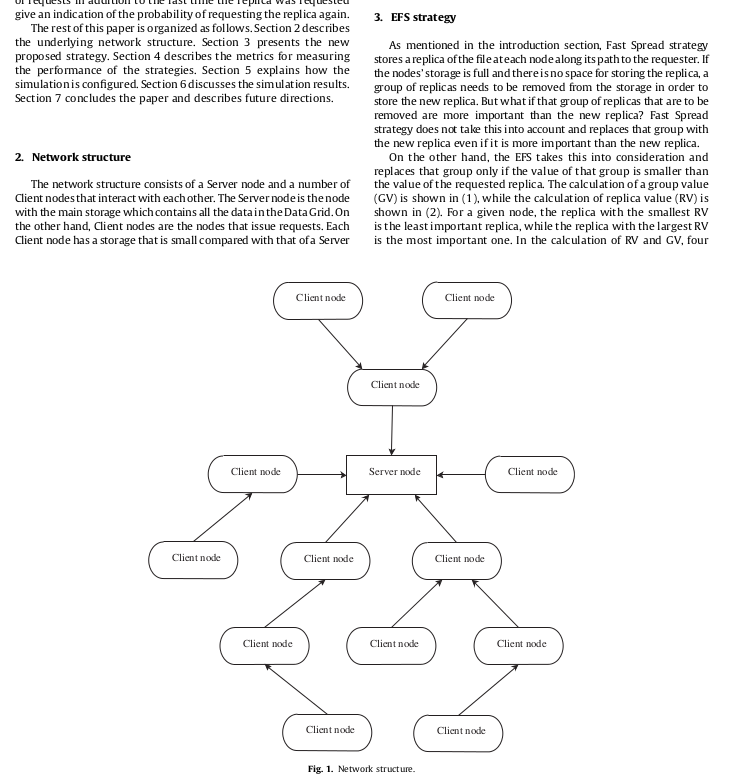
\includegraphics[width=13.4cm]{article_2011_sample.png}}
  \end{center}
  \caption{Izsek iz članka \cite{efs2011}.}
  \label{pic2011}
\end{figure}

\begin{figure}
  \begin{center}
    \fbox{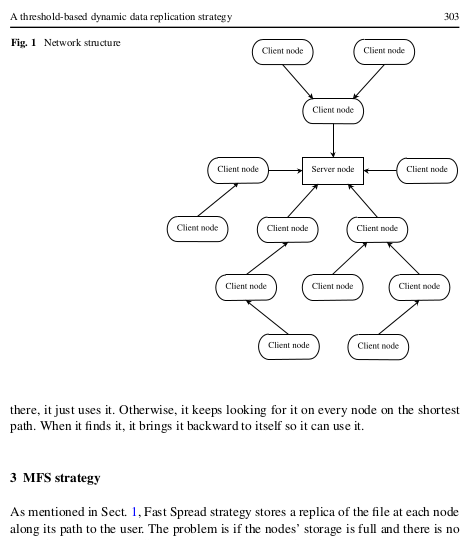
\includegraphics[width=13.4cm]{article_2012_sample.png}}
  \end{center}
  \caption{Izsek iz članka \cite{mfs2012}.}
  \label{pic2012}
\end{figure}



\chapter{Primerjava strategij iz člankov}

\section{Opis strategij zamenjave}
Kot je že bilo omenjeno v razdelku~\ref{sec:fspread}, strategija Fast Spread
shrani zahtevano repliko na vsakem vozlišču na poti od vozlišča, kjer je
bila zahtevana replika najdena, do vozlišča, ki je repliko prvotno
zahtevalo. Če določeno vozlišče nima dovolj razpoložljivega prostora,
da bi zahtevano repliko shranilo, mora najprej izbrisati eno ali več
obstoječih replik.

Avtorji člankov opozarjajo, da je lahko skupina replik, ki jih je potrebno
izbrisati, pomembnejša od nove replike. Izpostavljajo,
da strategija Fast Spread tega ne upošteva in da zamenjavo skupine obstoječih
replik z novo repliko vedno izvede ne glede na morebitno večjo vrednost skupine
replik \cite{efs2011, mfs2012}.

Avtorji v obeh člankih predlagajo nekoliko spremenjeni različici strategije
Fast Spread, pri katerih se zamenjava izvede le v primerih, ko je vrednost
skupine replik strogo manjša od vrednosti nove replike. Strategiji pri tem
za ocenjevanje vrednosti (skupin) replik uporabljata metrike, opisane v
nadaljevanju.

\subsection{Strategija EFS}

Strategija EFS je opisana v članku \cite{efs2011}. Njena psevdokoda
je prikazana na sliki psevdokoda~\ref{alg:EFS}, pri čemer
je pomen posameznih spremenljivk pojasnjen v tabeli~\ref{tbl:EFS_vars}.

\begin{algorithm}
  \label{alg:EFS}
  \caption{Strategija EFS. Vir: \cite{efs2011}.}

  \SetKwComment{blankln}{}{}

  Initialize SOS to $0$\;
  \eIf{RR exists on RN}{
      Use RR\;
  }{
      \For{$i = 2$ \KwTo NSPList.size}{
          \If{RR exists on NSPList(i)}{
              \For{$j = \mathit{NSPList}(i - 1)$ \KwTo $1$}{
                  \eIf{CNFSS $\geq$ RR.Size}{
                      Copy RR\;
                  }{
                      \For{$x = 1$ \KwTo ReplicaList.size}{
                          \eIf{$\mathit{SOS} + \mathit{CNFSS} <$ RR.Size}{
                              SOS = SOS + \textit{SizeList(x)}\;
                          }{
                              Break\;
                          }
                      }

\blankln{}

                      $\mathit{GV} = \frac{\sum_{y=1}^{x-1}
                          \mathit{NORList(y)}}{
                                  \sum_{y=1}^{x-1} \mathit{SizeList(y)}} +
                          \frac{\sum_{y=1}^{x-1}
                              \mathit{NORFSTIList(y)}}{\mathit{FSTI}} +
                          \frac{1}{\mathit{CT} - \frac{\sum_{y=1}^{x-1}
                              \mathit{LRTList(y)}}{x-1}}$

\blankln{}

                      $\mathit{RV_{RR}} =
                          \frac{\mathit{NORRR}}{\mathit{SRR}} +
                          \frac{\mathit{NORRRFSTI}}{\mathit{FSTI}} +
                          \frac{1}{\mathit{CT} - \mathit{LRTRR}}$

\blankln{}

                      \If{$\mathit{GV} < \mathit{RV_{RR}}$} {
                          \For{$y = 1$ \KwTo $x-1$}{
                            Delete \textit{ReplicaList(y)},
							  \textit{NORList(y)},
							  \textit{SizeList(y)}, \textit{NORFSTIList(y)},
							  \textit{LRTList(y)}\;
                          }
                          Copy RR;
                      }
                  }
              }
          }
      }
  }
\end{algorithm}

\begin{table}
\small
  \begin{center}
    \begin{tabulary}{1.0\textwidth}{ >{\itshape}p{6.8em} p{26em}}
      \textnormal{Spremenljivka} & Pomen \\
      \hline
      RR & zahtevana replika \\
      RN &  vozlišče, ki zahteva repliko \\
      CNFSS & velikost nezasedenega prostora na trenutno opazovanem
          \mbox{vozlišču} \\
      FSTI & frekvenčnospecifičen časovni interval (največja starost
         zahtevkov, do katere jih še štejemo kot zahtevke iz bližnje
         preteklosti) \\
      NORRR & število zahtevkov za \textit{RR} \\
      SRR & velikost \textit{RR} \\
      NORRRFSTI & število zahtevkov za zahtevano repliko
          v \textit{FSTI} \\
      CT & trenutni čas \\
      LRTRR & čas zadnjega zahtevka za zahtevano repliko \\
      SOS & spremenljivka, ki predstavlja vsoto velikosti skupine replik na
          trenutno opazovanem vozlišču \\
      NSPList & seznam vozlišč na najkrajši poti od \textit{RN} do
          glavnega strežnika \\
      ReplicaList & seznam obstoječih replik na trenutno opazovanem vozlišču,
          urejenih po naraščajočem vrstnem redu glede na njihovo vrednost
          \textit{RV}. Če ima več replik enako vrednost \textit{RV}, so med
          seboj urejene naključno. \\
      NORList & seznam, ki vsebuje vrednosti, kolikokrat je istoležne
          replike s seznama \textit{ReplicaList} zahtevalo
          trenutno opazovano vozlišče. \\
      SizeList & seznam, ki vsebuje velikosti istoležnih replik s seznama
          \textit{ReplicaList} \\
      NORFSTIList & seznam, ki vsebuje vrednosti, kolikokrat je istoležne
          replike s seznama \textit{ReplicaList} v intervalu \textit{FSTI}
          zahtevalo trenutno opazovano vozlišče  \\
      LRTList & seznam, ki vsebuje čase zadnjega zahtevka za istoležne
          replike s seznama \textit{ReplicaList}
    \end{tabulary}
 \end{center}

  \caption{Pomen spremenljivk v psevdokodi strategije EFS. Vir: \cite{efs2011}.}
  \label{tbl:EFS_vars}
\end{table}

Kadar neko vozlišče prejme zahtevano repliko, za shranitev katere nima dovolj
nezasedenega prostora (vrstica~10), pogleda, koliko
obstoječih replik bi zaradi tega moralo predhodno izbrisati. Sprehodi se skozi
seznam~\textit{\mbox{ReplicaList}}, dokler vsota velikosti obiskanih replik in
velikosti nezasedenega prostora ne doseže (ali preseže) velikosti nove replike
(vrstice 11--17). Vse obiskane replike nato implicitno
tvorijo skupino replik, ki bodo potencialno izbrisane.

Vozlišče v nadaljevanju izračuna vrednosti nove replike in skupine replik
(vrstici~18~in~19) ter ju med seboj primerja. Če je
vrednost skupine manjša (vrstica~20), vozlišče izbriše vse replike
iz skupine in njihove statistike ter jih nadomesti z novo repliko
(vrstice~21--24).

Strategija EFS pri ocenjevanju vrednosti replik upošteva naslednje štiri
stvari:
\begin{itemize}
  \item število zahtevkov za repliko,
  \item pogostost zahtevkov,
  \item velikost replike,
  \item čas od zadnjega zahtevka za repliko.
\end{itemize}

Število zahtevkov, njihova pogostost in čas od zadnjega zahtevka so pomembni
dejavniki, saj z njihovo pomočjo lahko ocenimo verjetnost, da bo replika
v prihodnosti ponovno zahtevana. Ker imajo vozlišča omejen prostor za
shranjevanje, je pomembna tudi velikost replik.

\begin{samepage}
Iz vrstice~19 psevdokode~\ref{alg:EFS} lahko razberemo
formulo za izračun vrednosti posamezne replike:
\begin{equation}
  \mathit{RV} = \frac{\mathit{NORRR}}{\mathit{SRR}} +
                      \frac{\mathit{NORRRFSTI}}{\mathit{FSTI}} +
                      \frac{1}{\mathit{CT} - \mathit{LRTRR}}
  \label{eq:EFS_RV}
\end{equation}
Pomen posameznih spremenljivk je pojasnjen v tabeli~\ref{tbl:EFS_vars}.
\end{samepage}

Iz prvega in drugega člena enačbe~\eqref{eq:EFS_RV} je razvidno, da imajo
višjo vrednost tiste replike, ki so bile večkrat zahtevane (večje število
zahtevkov), pri čemer drugi člen upošteva zgolj zahtevke iz nedavne zgodovine,
torej znotraj intervala FSTI, ki jih dodatno normira z velikostjo tega
intervala. Iz prvega člena je tudi razvidno, da je vrednost replik obratno
sorazmerna z njihovo velikostjo. Večje replike so vrednotene niže, saj
zasedajo več prostora na vozlišču. Zadnji člen daje višjo vrednost replikam,
katerih čas od njihovega zadnjega zahtevka je manjši.

\begin{samepage}
Podobno kot vrednost posamezne replike se izračuna tudi vrednost skupine
replik, in sicer po formuli iz vrstice~18 v psevdokodi~\ref{alg:EFS}:
\begin{equation}
  \mathit{GV} = \frac{\sum\limits_{y=1}^{x-1} \mathit{NORList(y)}}{
                      \sum\limits_{y=1}^{x-1} \mathit{SizeList(y)}} +
                \frac{\sum\limits_{y=1}^{x-1} \mathit{NORFSTIList(y)}}{
                      \mathit{FSTI}} +
                \frac{1}{\mathit{CT} - \frac{\sum\limits_{y=1}^{x-1}
                         \mathit{LRTList(y)}}{x-1}}
  \label{eq:EFS_GV}
\end{equation}
Pomen posameznih spremenljivk pojasnjen v tabeli~\ref{tbl:EFS_vars}.
\end{samepage}
\vspace{0.5em}

Enačbi~\eqref{eq:EFS_RV}~in~\eqref{eq:EFS_GV} sta vsebinsko gledano
pravzaprav enaki. Edina razlika je, da so posamezni členi iz
enačbe~\eqref{eq:EFS_RV} v enačbi~\eqref{eq:EFS_GV} namesto za posamezno
repliko izračunani na ravni celotne skupine replik.
Tako je med drugim v prvem členu enačbe~\eqref{eq:EFS_GV} izračunano razmerje
med skupnim številom zahtevkov in skupno velikostjo \textit{vseh replik} iz
skupine, v tretjem členu pa je uporabljen \textit{povprečen čas} od zadnjega
zahtevka za posamezno repliko v skupini.


\subsection{Strategija MFS}

Strategija MFS je opisana v članku~\cite{mfs2012}. Njena
psevdokoda je prikazana na sliki psevdokoda~\ref{alg:MFS} in razvidno je,
da je v konceptu skoraj popolnoma enaka strategiji~EFS. Od nje se razlikuje
zgolj v formulah za izračun vrednosti replike in vrednosti skupine replik
ter v vrstnem redu, po katerem so replike urejene v seznamu
\textit{ReplicaList}.

\begin{samepage}
Vrednost replike se izračuna po naslednji formuli iz vrstice~11
v psevdokodi~\ref{alg:MFS}:
\begin{equation}
  \mathit{PNOR} = \mathit{NOR} \times
                  \frac{\mathit{RR.Size} - \mathit{CNFSS}}{
                        \mathit{ RR.Size}}
  \label{eq:MFS_RV}
\end{equation}
Pomen posameznih spremenljivk je pojasnjen v tabeli~\ref{tbl:MFS_vars}.
\end{samepage}
\vspace{1em}

Vrednost replike je PNOR (``delno število zahtevkov''). Izračuna
se kot skupno število zahtevkov za repliko (NOR), prilagojeno za
korekcijski faktor. Slednji je odvisen od razmerja med velikostjo replike
in velikostjo nezasedenega prostora na vozlišču. V robnem primeru,
ko je ves razpoložljiv prostor na vozlišču zaseden (CNFSS je enak 0), sta
vrednosti PNOR in NOR enaki.

PNOR ni nikoli negativno število. Ulomek v enačbi~\eqref{eq:MFS_RV} je namreč
vedno pozitiven, saj je tudi njegov imenovalec pozitiven~---~velikost replike
\textit{RR.Size} je namreč strogo večja od velikosti nezasedenega prostora
\textit{CNFSS}. Če bi bilo obratno, bi namreč vozlišče repliko takoj shranilo
in niti ne bi šlo računati njene vrednosti, kar je razvidno iz vrstic~8~in~9
psevdokode~\ref{alg:MFS}.

\begin{samepage}
Vrednost skupine replik se izračuna po formuli, ki se nahaja na levi strani
neenakosti v vrstici~19:
\begin{equation}
	\sum\limits_{y=1}^{x-1} \mathit{NORList(y)}
  \label{eq:MFS_GV}
\end{equation}
Pomen posameznih spremenljivk je pojasnjen v tabeli~\ref{tbl:MFS_vars}.
\end{samepage}
\vspace{1em}

Formula~\eqref{eq:MFS_GV} je zelo enostavna, saj zgolj sešteje število
zahtevkov (NOR) za vse replike, ki sestavljajo skupino.

Kot že omenjeno, se strategija MFS od strategije EFS nekoliko razlikuje
tudi v tem, iz katerih replik vozlišče sestavi skupino replik, ki bodo morda
zamenjane. Razlog za to je različna urejenost replik v seznamu
\textit{ReplicaList}. Medtem ko strategija EFS replike uredi glede na
njihovo vrednost (RV), jih strategija MFS uredi glede na
število zahtevkov zanje, v primeru enakih vrednosti pa še dodatno
glede na njihovo velikost. Urejenost seznama \textit{ReplicaList} je
sicer opisana tudi v tabelah~\ref{tbl:EFS_vars}~oziroma~\ref{tbl:MFS_vars}.

\vspace{2cm}
\begin{algorithm}[H]
  \label{alg:MFS}
  \caption{Strategija MFS. Vir: \cite{mfs2012}.}

  \SetKwComment{blankln}{}{}

  Initialize SOS to $0$\;
  \eIf{RR exists on RN}{
      Use RR\;
  }{
      \For{$i = 2$ \KwTo NSPList.size}{
          \If{RR exists on NSPList(i)}{
              \For{$j = \mathit{NSPList}(i - 1)$ \KwTo $1$}{
                  \eIf{CNFSS $\geq$ RR.Size}{
                      Copy RR\;
                  }{
                      $\mathit{PNOR} =
                          \mathit{NOR} \times
                          \tfrac{\mathit{RR.Size} - \mathit{CNFSS}}{
                                 \mathit{ RR.Size}}$

                      \For{$x = 1$ \KwTo ReplicaList.size}{
                          \eIf{SOS $<$ RR.Size $- \mathit{CNFSS}$}{
                              SOS = SOS + \textit{SizeList(x)}\;
                          }{
                              Break\;
                          }
                      }

                      \If{$\sum_{y=1}^{x-1} \mathit{NORList(y)} <
                          \mathit{PNOR}$} {
                          \For{$y = 1$ \KwTo $x-1$}{
                              Delete \textit{ReplicaList(y)},
                              \textit{SizeList(y)}, \textit{NORList(y)}\;
                          }
                          Copy RR;
                      }
                  }
              }
          }
      }
  }
\end{algorithm}


\begin{table}
\small
  \begin{center}
    \begin{tabulary}{1.0\textwidth}{ >{\itshape}p{6.8em} p{26em}}
      \textnormal{Spremenljivka} & Pomen \\
      \hline
      RR & zahtevana replika \\
      RN &  vozlišče, ki zahteva repliko \\
      CNFSS & velikost nezasedenega prostora na trenutno opazovanem
          \mbox{vozlišču} \\
      NOR & število zahtevkov za \textit{RR} \\
      PNOR & delno število zahtevkov za \textit{RR} \\
      SOS & spremenljivka, ki predstavlja vsoto velikosti skupine replik na
          trenutno opazovanem vozlišču \\
      NSPList & seznam vozlišč na najkrajši poti od \textit{RN} do
          glavnega strežnika \\
      ReplicaList & seznam obstoječih replik na trenutno opazovanem vozlišču,
          urejenih po naraščajočem vrstnem redu glede na njihovo vrednost
          \textit{NOR}.
          Če ima več replik enako vrednost \textit{NOR}, so med seboj
          urejene v padajočem vrstnem redu glede na njihovo velikost. Če so
          tudi velikosti enake, je medsebojni vrstni red teh replik
          naključen. \\
      SizeList & seznam, ki vsebuje velikosti istoležnih replik s seznama
          \textit{ReplicaList} \\
      NORList & seznam, ki vsebuje vrednosti, kolikokrat je istoležne
          replike s seznama \textit{ReplicaList} zahtevalo trenutno opazovano
          vozlišče. \\
    \end{tabulary}
  \end{center}

  \caption{Pomen spremenljivk v psevdokodi strategije MFS. Vir: \cite{mfs2012}.}
  \label{tbl:MFS_vars}
\end{table}


\section{Implementacija diskretne simulacije}

Za preizkus strategij, opisanih v člankih, sem v programskem jeziku Python
(različica 3.3) napisal diskretno simulacijo. S poganjanjem slednje z
raz\-ličnimi parametri sem lahko primerjal, kako se obnesejo posamezne
strategije zamenjave. Glavni sestavni deli simulacije so vozlišča, replike,
dogodki v simulaciji in sámo izvajalno okolje simulacije \cite{plamut_github}.

Topologija podatkovnega omrežja, ki sem jo uporabil, je polni graf, saj so
takšno topologijo izbrali tudi avtorji člankov \cite{efs2011, mfs2012}.
Povezave med vsakim parom vozlišč so simetrične, njihove dolžine pa se v fazi
inicializacije simulacije naključno določijo. V isti fazi se generirajo tudi
replike naključnih velikosti.

Ko so dolžine povezav med vozlišči določene, se na grafu, ki predstavlja
podatkovno omrežje, izvede algoritem Dijkstra, ki poišče najkrajše poti med
glavnim strežnikom in vsemi ostalimi vozlišči. Po izvedbi algoritma vsakemu
vozlišču določimo, kdo je njegov starš na najkrajši poti do glavnega strežnika.
Slednji je pri tem seveda izjema, saj se nahaja povsem na vrhu hierarhije in
zato starša nima.

Med izvajanjem simulacije je vsako vozlišče avtonomno in se samo odloča, katere
replike bo hranilo pri sebi, pri čemer sledi vnaprej določeni strategiji
zamenjave. V posamezni izvedbi simulacije vsa vozlišča uporabljajo enako
strategijo in je med izvajanjem ne spreminjajo.

\subsection{Vrste dogodkov v simulaciji}
V okviru simulacije so definirane naslednje štiri vrste dogodkov, ki se lahko
pojavijo v njej:

\begin{itemize}
  \item \textbf{Pošlji zahtevek za repliko:} Vozlišče svojemu staršu pošlje
  zahtevek za repliko, ki je sámo nima. Posledično se za starša po določeni
  zakasnitvi sproži dogodek \textit{prejmi zahtevek za repliko}.

  \item \textbf{Prejmi zahtevek za repliko:} Vozlišče prejme zahtevek za
  določeno repliko od enega izmed svojih sinov. Če repliko ima, sproži dogodek
  \textit{pošlji repliko}, sicer pa posreduje zahtevek za isto repliko
  naprej svojemu staršu in s tem sproži dogodek \textit{pošlji zahtevek za
  repliko}.

  Če vir zahtevka ni določen, to označuje, da je zahtevek ustvarilo kar
  vozlišče sámo. Če zahtevano repliko že ima pri sebi, jo enostavno
  uporabi in se v simulaciji zaradi tega ne zgodi nič, sicer pa repliko
  zahteva od svojega starša.

  \item \textbf{Pošlji repliko:} Vozlišče začne pošiljati repliko tja, od
  koder je bila od njega zahtevana. Po določeni zakasnitvi se sproži ustrezen
  dogodek \textit{prejmi repliko}.

  \item \textbf{Prejmi repliko:} Replika prispe do vozlišča, ki je poslalo
  zahtevek zanjo. Če je vozlišče repliko zahtevalo zato, ker jo je predhodno
  od njega zahtevalo neko drugo vozlišče, jo temu vozlišču posreduje naprej.
  V tem primeru se sproži nov dogodek \textit{pošlji repliko}.
\end{itemize}

Pri dogodku \textit{prejmi zahtevek za repliko} je potrebno omeniti, da se
lahko pojavi tudi takrat, ko je vozlišče isto repliko že zahtevalo in trenutno
čaka, da jo prejme od starša. Ne glede na to vozlišče tudi v tem primeru staršu
pošlje nov zahtevek za isto repliko. Strategiji \ref{alg:EFS} in \ref{alg:MFS}
namreč ne predvidevata, da vozlišče vodi seznam replik, na prejem katerih
že čaka, temveč se vozlišče odloča zgolj na podlagi tega, ali v določenem
trenutku zahtevano repliko ima pri sebi ali ne.

Med izvajanjem simulacije posamezna vozlišča naključno in neodvisno drugo od
drugega sprožajo nove zahtevke za replike. Vse skupaj poteka v izvajalnem
okolju simulacije, ki skrbi za generiranje teh naključnih dogodkov, za
pravilno razporejanje dogodkov v časovni vrsti, za procesiranje dogodkov,
ko pridejo na vrsto, in za beleženje različnih statistik.

Izvajalno okolje skrbi tudi za pravilne zakasnitve dogodkov, ki so že uvrščeni
v časovno vrsto, kadar je to potrebno. Primer tega je dogodek
\textit{pošlji repliko}, ki povzroči, da se trajanje prenosov replik, ki
jih vozlišče že pošilja, podaljša. Replike se namreč pošiljajo sočasno in si
enakomerno delijo pasovno širino, ki je vozlišču na voljo. Posledično mora
izvajalno okolje ob začetku pošiljanja nove replike ustrezno zakasniti vse
dogodke tipa \textit{prejmi repliko}, na katere to vpliva.


\section{Meritve}
\subsection{Priprava simulacije}

Simulacijo sem pripravil na enak način, kot je opisan v obeh člankih, in v
njej med seboj primerjal štiri strategije zamenjave --- LRU, LFU, EFS in MFS.
Za ocenjevanje strategij sem uporabil predlagani metriki, in sicer skupen
odzivni čas in skupno porabo pasovne širine (tabela~\ref{tbl:sim_metrics}).
Dobra strategija obe metriki minimizira.

Odzivni čas je definiran kot čas, ki preteče od trenutka, ko vozlišče pošlje
zahtevek za repliko, do trenutka, ko zahtevano repliko prejme. Pri tem
predpostavimo, da je čas, potreben za obdelovanje zahtevka in morebitno
zamenjavo replik, zanemarljivo majhen. Če ima vozlišče želeno repliko že
pri sebi, je odzivni čas enak nič.

Porabljena pasovna širina je količina podatkov, ki jih je potrebno prenesti
takrat, kadar vozlišče zahteva repliko, ki je nima shranjene lokalno. Pri
tem se šteje, da je ta količina kar enaka velikosti zahtevane replike.

Ker sta pričakovani vsoti vseh odzivnih časov in velikosti vseh prenesenih
replik zelo veliki, sta obe metriki pomnoženi s konstantama $C_1$ in $C_2$,
ki zmanjšata njuni vrednosti. Vrednost obeh konstant je nastavljena na
$0,001$.

\begin{table}
\small
  \begin{center}
    \begin{tabulary}{1.0\textwidth}{ >{\itshape}p{9em} J}
      \textnormal{Metrika} & Opombe \\
      \hline
      $M_1 = \mathit{TRT} \times C_1$ &
        \textit{TRT}: skupen odzivni čas, $C_1$: konstanta \\
      $M_2 = \mathit{TBC} \times C_2$ &
        \textit{TBC}: skupna porabljena pasovna širina, $C_2$: konstanta
    \end{tabulary}
  \caption{Metriki za ocenjevanje uspešnosti strategij.
    Vir: \cite{efs2011,mfs2012}.}
  \end{center}

  \label{tbl:sim_metrics}
\end{table}

Replike so kategorizirane v skupine, in sicer tako, da je v vsaki skupini
enako število replik in da vsaka replika pripada zgolj eni skupini.%
\footnote{Kategorizacija replik v skupine ni v nobeni povezavi s tisto skupino
replik, ki jo določeno vozlišče tvori vsakokrat, ko se med izvajanjem
simulacije odloča, katere replike bo morda zamenjalo z novo repliko.}
Število vseh skupin je deset, tako da vsaka izmed njih vsebuje 10~\% replik.

Vsako vozlišče ima svojo t.~i.~\textit{najbolj želeno skupino} (MWG).
Verjetnost, da vozlišče zahteva določeno repliko, ki pripada njegovi skupini
MWG, je višja od verjetnosti, da zahteva določeno drugo repliko, ki pripada
eni izmed ostalih skupin. To je namreč boljši približek situacijam v praksi,
kjer se dostikrat zgodi, da se določena podmnožica podatkov (replik) v
primerjavi z ostalimi podatki veliko bolj pogosto uporablja
\cite{efs2011, mfs2012}.

Strategije sem med seboj primerjal v treh različnih scenarijih:
\begin{itemize}
  \item \textbf{Scenarij 1:} Vozlišče zahteva vse replike z
    enako verjetnostjo. To pomeni, da je verjetnost, da zahteva repliko iz
    svoje skupine MWG, zgolj 0,10 --- torej enaka, kot verjetnost za
    katerokoli drugo skupino replik.

  \item \textbf{Scenarij 2:} Vozlišče zahteva eno izmed replik iz svoje
    skupine MWG z verjetnostjo 0,30. To pomeni, da je verjetnost, da
    zahteva repliko iz ene izmed ostalih skupin, enaka 0,70.

  \item \textbf{Scenarij 3:} Vozlišče zahteva eno izmed replik iz svoje
    skupine MWG z verjetnostjo 0,50, z enako verjetnostjo pa tudi repliko
    iz ene izmed ostalih skupin.
\end{itemize}
V vsakem izmed naštetih scenarijev simulacijo poženemo enkrat za vsako
strategijo, kar skupaj znese 12 izvedb simulacije
(3 scenariji $\times$ 4 strategije). V posamezni izvedbi vsa vozlišča
uporabljajo enako strategijo --- tisto, ki jo takrat preizkušamo.

Nastavitve simulacije se med izvedbami ne spreminjajo. Uporabljene vrednosti
parametrov prikazuje Tabela~\ref{tbl:sim_params}.
Velikosti replik, časi med prihodi zahtevkov vozlišč in oddaljenosti med
vozlišči imajo enakomerno diskretno porazdelitev. Zavzamejo lahko katerokoli
celoštevilčno vrednost znotraj njihovega intervala možnih vrednosti.


\begin{table}
\small
  \begin{center}
    \begin{tabulary}{1.0\textwidth}{ p{16.7em} @{\extracolsep{2em}} p{15.8em}}
      \textnormal{Parameter} & Vrednost \\
      \hline
      Število vozlišč & 20 \\
      Število replik & 1000 \\
      Velikost vsake replike & med 100 in 1000 Mbit \\
      Število generiranih zahtevkov & \numprint{100000} \\
      Čas med prihodi zahtevkov vozlišč & med 0 in 99 s \\
      Število skupin replik & 10 \\
      Diskovni prostor na vozliščih (razen glavnega strežnika) &
          \numprint{50000} Mbit \\
      Diskovni prostor na glavnem strežniku & dovolj velik, da lahko naenkrat
          hrani vse replike podatkovnega omrežja \\
      Število replik v vsaki skupini & 100 \\
      Pasovna širina omrežja & 10 Mbit/s \\
      Razdalja med vsakim parom neposredno povezanih vozlišč &
        med 1 in 1000 km \\
      Hitrost širjenja signala po mrežnih povezavah & $6 \times 10^3$ km/s \\
      Frekvenčnospecifičen časovni interval (največja starost
         zahtevkov, do katere jih še štejemo kot zahtevke iz bližnje
         preteklosti) & \numprint{10000} \\
      C1 & 0,001 \\
      C2 & 0,001
    \end{tabulary}
  \end{center}

  \caption{Parametri simulacije in njihove vrednosti.
    Vir: \cite{efs2011,mfs2012}.}
  \label{tbl:sim_params}
\end{table}



\subsection{Rezultati simulacij}

Rezultati simulacij so prikazani na
slikah~\ref{hist_rsp_t}~in~\ref{hist_bw_used}. Po pričakovanjih
sta bila odzivni čas in porabljena pasovna širina manjša v scenarijih~2~in~3,
saj tam vozlišča določene skupine replik bolj pogosto zahtevajo, zato so
koristi od njihovega lokalnega hranjenja večje.

Presenetljivo je dejstvo, da sta strategiji EFS in MFS dosegli
\textit{identične} rezultate. Prva misel je seveda bila, da je šlo za napako v
implementaciji, vendar pa se je z analizo, opisano v
razdelkih~\ref{ss:EFS_bad}~in~\ref{ss:MFS_bad},
izkazalo, da je vzrok že v sami zasnovi omenjenih strategij.

Dobljeni rezultati tudi močno odstopajo od tistih, ki jih v člankih
navajajo avtorji \cite{efs2011,mfs2012}. Trend razlik med rezultati posameznih
scenarijev je sicer podoben, vendar so izmerjene vrednosti občutno drugačne.
Razvidno je tudi, da predlagani strategiji v nasprotju s trditvami avtorjev ne
dosežeta praktično nobenega izboljšanja v primerjavi s strategijo~LRU in celo
zaostajata za strategijo~LFU. Možne razlage za vse navedene razlike so opisane v
razdelku~\ref{s:results_mismatch}.

\begin{figure}
\begin{tikzpicture}[scale=1.2]
  \begin{axis}[
    ybar,
    ylabel={Skupen odzivni čas [s]},
    enlarge x limits=0.3,
    try min ticks=7,
    ytick pos=left,
    scaled y ticks = false,
    ymin = 0,
    y label style={
        at={(-0.1,0.5)}
    },
    yticklabel style={%
        /pgf/number format/fixed
    }, 
    xtick style={white},  % efectively remove the tick marks
    xtick=data,
    xticklabels={Scenarij 1, Scenarij 2, Scenarij 3},
    xtick align=inside,
    bar width=10pt,
    area legend,
    legend style={
        draw=none    % remove the box around the legend
    }
  ]

    \addplot[fill=gray!40] coordinates {  % LRU
      (1, 55268.55) (2, 40752.71) (3, 24122.26)
    };
    \addplot[fill=gray] coordinates {  % LFU  
      (1, 41110.83) (2, 27399.93) (3, 15091.31)
    };
    \addplot[fill=black] coordinates {  % EFS 
      (1, 52726.21) (2, 38396.94) (3, 23142.42)
    };    
    \addplot[fill=white] coordinates {  % MFS
      (1, 52726.21) (2, 38396.94) (3, 23142.42)
    };
        
    \legend{LRU, LFU, EFS, MFS}

  \end{axis}
\end{tikzpicture}

\caption{Skupen odzivni čas glede na uporabljeno strategijo.}
\label{hist_rsp_t}
\end{figure}



\begin{figure}
\begin{tikzpicture}[scale=1.2]
  \begin{axis}[
    ybar,
    ylabel={Porabljena pasovna širina [Mbit]},
    enlarge x limits=0.3,
    try min ticks=7,
    ytick pos=left,
    scaled y ticks=false,
    ymin = 0,
    y label style={
        at={(-0.1,0.5)}
    },
    yticklabel style={%
        /pgf/number format/fixed
    },    
    xtick style={white},  % efectively remove the tick marks
    xtick=data,
    xticklabels={Scenarij 1, Scenarij 2, Scenarij 3},
    xtick align=inside,
    bar width=10pt,
    area legend,
    legend style={
        at={(-0.15, -0.15)},
        anchor=north west,
        legend columns=-1,
        column sep=0.1cm,
        /tikz/every even column/.append style={column sep=0.3cm}
    }
  ]

    \addplot[fill=gray!40] coordinates {  % LRU
      (1, 111905.38) (2, 107773.46) (3, 97338.32)
    };
    \addplot[fill=gray] coordinates {  % LFU  
      (1, 109987.49) (2, 101329.39) (3, 81382.90)
    };
    \addplot[fill=black] coordinates {  % EFS 
      (1, 111580.25) (2, 106975.95) (3, 96241.67)
    };    
    \addplot[fill=white] coordinates {  % MFS
      (1, 111580.25) (2, 106975.95) (3, 96241.67)
    };
        
    \legend{LRU, LFU, EFS, MFS}

  \end{axis}
\end{tikzpicture}

\caption{Skupno porabljena pasovna širina glede na uporabljeno strategijo.}
\label{hist_bw_used}
\end{figure}


\chapter{Kritična presoja člankov}

\section{Sum recikliranja}

Članka sta si že na prvi pogled zelo podobna. Oba imata \textit{identično}
strukturo, naslovi razdelkov in podrazdelkov so, razen imena opisane
strategije, popolnoma enaki. V obeh člankih je uporabljena ista slika sheme
podatkovnega omrežja in tudi velik del besedila v člankih je skorajda
popolnoma enak. Kot primer si poglejmo prvi odstavek drugega razdelka
v članku~\cite{efs2011}:

\begin{itquote}
The network structure consists of a Server node and a number of
Client nodes that interact with each other. The Server node is the node
with the main storage which contains all the data in the Data Grid. On
the other hand, Client nodes are the nodes that issue requests. Each
Client node has a storage that is small compared with that of a Server
node and thus cannot accommodate all the requested replicas.
Therefore, some of the replica requests are served non-locally.
\end{itquote}

Primerjajmo ga s prvim odstavkom drugega razdelka v članku~\cite{mfs2012}:

\begin{itquote}
The employed network structure consists of a Server node and a number of
Client nodes that interact with each other as appears in Fig. 1. The Server
node is the node with the main storage which contains all the data that
belongs to the Data Grid. On the other hand, Client nodes are the nodes that
create the requests. Each of these nodes includes a storage that is relatively
small if compared with the Server node’s storage and cannot hold all the
requested replicas. Thus, some of the requested replicas are brought from the
other nodes.
\end{itquote}

Oba citirana odstavka vsebujeta skorajda enake stavčne strukture. Razlikujeta
se zgolj v tem, da so nekatere besede in besedne zveze nadomeščene s
sopomenkami oziroma z nekoliko drugačnimi besednimi zvezami, ki pa pomena
stavkov ne spremenijo.

Citirana odstavka še zdaleč nista edini primer, pravzaprav je skorajda
celotno besedilo obeh člankov sestavljeno iz takšnih parov medsebojno podobnih
odstavkov. Domnevamo lahko, da so avtorji vnesli določene spremembe v besedilo
novejšega izmed člankov zgolj zato, da bi se izognili morebitni samodejni
zaznavi podvojenih člankov s strani temu namenjenih programov.

\section{Neujemanje rezultatov}
\label{s:results_mismatch}

Rezultati, pridobljeni s simulacijo, se močno razlikujejo od tistih,
predstavljenih v člankih. Po trditvah avtorjev se strategiji EFS in MFS
obneseta veliko bolje od strategij LRU in LFU, vendar pa tega ni bilo možno
ponoviti.

Splošni trendi med posameznimi scenariji se sicer ujemajo. Večja kot je
verjetnost, da vozlišče zahteva eno izmed replik iz svoje skupine MWG, manjši
je skupen odzivni čas in porabljena pasovna širina, kar velja za vse štiri
preizkušene strategije. Slednje je nenazadnje tudi pričakovano, saj so v teh
primerih posamezne skupine replik bolj pogosto zahtevane in to dejstvo lahko
vozlišča s pridom izkoristijo pri odločanju, katere skupine replik je bolj
smiselno shraniti (in obdržati) tudi lokalno.

Po drugi strani pa je iz rezultatov očitno, da strategiji EFS in MFS ne
prineseta nobenega pravega izboljšanja glede na referenčni strategiji LRU in
LFU. Ker so vse obravnavane strategije med seboj v zasnovi enake in se med
seboj razlikujejo zgolj v metrikah za ocenjevanje vrednosti replik in skupin
replik, leži ključ do razumevanja dobljenih rezultatov simulacije ravno v
podrobni analizi teh metrik.


\subsection{Slabosti metrik v strategiji EFS}
\label{ss:EFS_bad}

\subsubsection{Vrednost replike}

Vrednost replike v strategiji EFS se izračuna po formuli~\eqref{eq:EFS_RV}.
Prvi člen predstavlja razmerje med številom zahtevkov za repliko in velikostjo
replike. Ker je število zahtevkov za vsako novo repliko enako nič\footnote{%
Pojasnilo, zakaj vzamemo ravno vrednost nič, je v
razdelku~\ref{ss:sim_bad_desc}}, je tudi vrednost tega člena nič.

Drugi člen predstavlja razmerje med številom zahtevkov za repliko v zadnjem
časovnem intervalu FSTI in velikostjo tega intervala. Ker število zahtevkov
v intervalu seveda ne more biti večje od števila vseh zahtevkov,
slednje pa je enako nič, je tudi vrednost drugega člena
formule~\eqref{eq:EFS_RV} enaka nič.

Vrednost tretjega člena je odvisna od tega, koliko časa je minilo
od zadnjega zahtevka za repliko. Manjši kot je ta čas, večja je vrednost člena.
Ker pa vozlišče ne vodi statistik za tiste replike, katerih kopij nima
shranjenih pri sebi, je ta čas enostavno najmanjši možen, torej nič (začetek
simulacije). Iz tabele~\ref{tbl:sim_params} je razvidno, da so replike v
povprečju velike približno 550 megabitov. Ker je kapaciteta vsakega vozlišča
\numprint{50000}~Mb, lahko eno vozlišče v povprečju shrani približno 90
replik, preden mu zmanjka razpoložljivega prostora.

V simulaciji se novi zahtevki v povprečju pojavljajo na približno vsakih
50~sekund (razvidno iz tabele~\ref{tbl:sim_params}), kar pomeni, da mora
najprej preteči vsaj 4500 sekund ($90 \times 50\:s$), preden vozlišče
zahteva repliko, ki je ne more več shraniti brez zamenjave skupine
že shranjenih replik. V praksi je ta čas še veliko večji, saj je statistično
gledano praktično nemogoče, da bi vseh prvih 90 zahtevkov poslalo eno in isto
vozlišče v podatkovnem omrežju. Pričakovana vrednost tretjega člena
formule~\eqref{eq:EFS_RV} (in s tem tudi vrednost replike) je tako veliko
manjša od $\frac{1}{\numprint{4500}}$.

\subsubsection{Vrednost skupine replik}

Vrednost skupine replik se izračuna po formuli~\eqref{eq:EFS_GV}. Tudi tu si
poglejmo, kakšne vrednosti lahko zavzame vsak izmed njenih členov.

Prvi člen predstavlja povprečno vrednost razmerja med številom zahtevkov in
velikostjo replike vseh replik v skupini. Vsaka replika v skupini je bila
zahtevana najmanj enkrat (takrat, ko jo je vozlišče prvič zahtevalo in shranilo
pri sebi), po drugi strani pa je njena največja velikost omejena na
1000 megabitov (tabela~\ref{tbl:sim_params}). To pomeni, da je vrednost
prvega člena formule~\eqref{eq:EFS_GV} najmanj \numprint{0.001}.

Drugi člen predstavlja razmerje med skupnim številom zahtevkov za vse replike
v skupini v zadnjem časovnem intervalu FSTI in velikostjo tega intervala.
Skupno število zahtevkov v tem intervalu seveda ne more biti nikoli večje od
skupnega števila vseh zahtevkov, po drugi strani pa velikost tega intervala,
uporabljena v simulaciji, znaša \numprint{10000} (tabela~\ref{tbl:sim_params}).
Navedeno pomeni, da je drugi člen formule~\eqref{eq:EFS_GV} od prvega manjši za
cel velikostni red in ima na končno vrednost skupine replik zanemarljivo
majhen vpliv.

Vrednost tretjega člena je odvisna od tega, koliko časa je v povprečju minilo
od zadnjega zahtevka za vsako izmed replik v skupini. V simulaciji je v
scenariju~3 verjetnost, da vozlišče zahteva repliko iz svoje
skupine MWG, enaka 0,50. Ker je v vsaki skupini 100 replik, je za vsako
izmed njih verjetnost, da jo vozlišče zahteva, enaka 0,005, kar je v
povprečju enkrat na vsakih 200 zahtevkov.

Čas med dvema zahtevkoma je enakomerno porazdeljen na intervalu [0, 99] sekund,
torej v povprečju znaša slabih 50 sekund. To pomeni, da vozlišče določeno
repliko iz skupine MWG v povprečju zahteva zgolj na približno vsakih
\numprint{10000} sekund ($200 \times 50\:\text{s}$).
Ker se ta vrednost nahaja v imenovalcu tretjega člena
formule~\eqref{eq:EFS_RV}, je njegova pričakovana vrednost okoli $10^{-4}$ (za
manj pogosto zahtevane replike pa še manjša), kar je za red velikosti manjše
od prvega člena iste formule.

Pri analizi obeh metrik v strategiji EFS sta pomemebni predvsem naslednji
ugotovitvi:
\begin{itemize}
\item Pri obeh metrikah je samo en člen formule tisti, ki dejansko določa
končno vrednost. Druga dva člena sta v primerjavi z njim zanemarljivo majhna.

\item Dominantni člen v formuli za izračun vrednosti replike je veliko manjši
od dominantnega člena v formuli za izračun vrednosti skupine replik.
\end{itemize}

Prva ugotovitev kaže na to, da metriki nista najbolje izbrani oziroma da
členi v njih morda niso ustrezno normirani. Druga ugotovitev pa razkriva še
večjo pomanjkljivost --- vrednost skupine replik v strategiji~EFS je vedno
večja od vrednosti nove replike!

Posledica je, da skupine obstoječih replik ne bodo nikoli zamenjane z novimi
replikami, zaradi česar se celotna strategija izrodi v nekakšno različico
statične replikacije. Pri tem je razporeditev replik v podatkovnem
omrežju bolj ali manj naključna, odvisna je namreč zgolj od
vrstnega reda pojavljanja zahtevkov za replike in ne sledi nobeni vnaprej
določeni hevristiki.


\subsection{Slabosti metrik v strategiji MFS}
\label{ss:MFS_bad}

\subsubsection{Vrednost replike}

Strategija MFS ocenjuje vrednosti replik po formuli~\eqref{eq:MFS_RV}.
Formulo lahko zapišemo tudi nekoliko drugače, in sicer števec ulomka delimo z
njegovim imenovalcem:

\begin{equation}
  \mathit{PNOR} = \mathit{NOR} \times
                 \left(1 - \frac{\mathit{CNFSS}}{\mathit{ RR.Size}}\right)
  \label{eq:MFS_RV_v2}
\end{equation}

Iz psevdokode~\ref{alg:MFS} je razvidno, da je velikost zahtevane replike
\textit{RR.Size} vedno večja od velikosti nezasedenega prostora na vozlišču
\textit{CNFSS} --- če to ne bi bilo res, bi vozlišče repliko enostavno shranilo
in sploh ne bi šlo ocenjevati njene vrednosti. Ulomek v
formuli~\eqref{eq:MFS_RV_v2} je zato manjši od ena, s tem pa vrednost izraza v
oklepaju zavzame vrednosti na intervalu (0,1].
Ker je število zahtevkov NOR za novo repliko kvečjemu enako
ena (odvisno sicer od tega, kako interpretiramo članek), tudi največja možna
vrednost replike po formuli~\eqref{eq:MFS_RV_v2} ni nikoli večja od te meje.

\subsubsection{Vrednost skupine replik}

Strategija MFS ocenjuje vrednosti skupin replik tako, da sešteje število
zahtevkov za vse replike v skupini (formula~\eqref{eq:MFS_GV}). Ker je
bila vsaka replika v skupini zahtevana vsaj enkrat (najmanj takrat, ko jo
je vozlišče zahtevalo in potem shranilo pri sebi), je vrednost skupine replik
vedno večja ali enaka ena.

Na podlagi povedanega je očitno, da vrednost skupine replik ni nikoli manjša
od vrednosti nove replike, s tem pa tudi pogoj za zamenjavo ni nikoli
izpolnjen. Ko se na vozliščih zapolni ves razpoložljivi prostor, le-ta
prenehajo shranjevati nove replike. Strategija MFS se po določenem času
izrodi v različico statične replikacije na enak način, kot se izrodi
tudi strategija EFS. Zdaj je tudi razumljivo, zakaj sta obe strategiji v
simulaciji dosegli popolnoma enake rezultate.


\section{Nejasnosti in druge napake v člankih}

Med razvojem simulacije se je izkazalo, da imata oba članka poleg vprašljivo
zastavljenih metrik tudi veliko drugih pomanjkljivosti. Ker določene stvari
niso dovolj podrobno opisane, se je bilo na nekaterih mestih
potrebno zanašati na določene predpostavke, ki pa so seveda lahko bile
drugačne od predpostavk avtorjev člankov.

Dvomljiva je tudi sama zasnova simulacije, kar velja tako za izbrane
vrednosti njenih parametrov kot tudi za izbiro topologije podatkovnega
omrežja, ki ne odraža nujno strukture tovrstnih omrežij v praksi.

Vse omenjene in še nekatere druge pomanjkljivosti so opisane v naslednjih
razdelkih.

\subsection{Pomanjkljiv opis posameznih delov simulacije}
\label{ss:sim_bad_desc}

\subsubsection{Manjkajoče enote nekaterih parametrov}

V tabeli, ki v člankih navaja vrednosti parametrov simulacije, ni podana
niti enota za čas med prihodi zahtevkov vozlišč niti enota za dolžino
časovnega intervala FTSI. Predpostavil sem, da gre v obeh primerih za sekunde,
saj je pasovna širina omrežja podana v količini prenesenih podatkov
\textit{na sekundo} (enota~\textit{Mbit/s}).

\subsubsection{Nepopoln opis uporabljene topologije omrežja}

Avtorji v člankih ne pojasnijo dovolj podrobno, na kakšni topologiji
podatkovnega omrežja so izvedli simulacijo. Navajajo zgolj to, da so uporabili
polni graf, v katerem vsako vozlišče pozna svojo najkrajšo pot do glavnega
strežnika in po tej poti tudi pošilja zahtevke za replike, ki jih nima lokalno
shranjenih.

Po drugi strani pa nič ne povedo o tem, kakšne so bile dejanske
razdalje med vozlišči. Zaradi tega ni možno izračunati omenjenih
najkrajših poti in posledično tudi ne določiti dejanske strukture omrežja.
Ta seveda vpliva na rezultate simulacije, saj ni vseeno, ali je veliko
vozlišč neposredno povezanih z glavnim strežnikom ali pa morajo replike
zahtevati posredno preko drugih vozlišč v omrežju.

\subsubsection{Dvoumen opis časa med prihodi zahtevkov in pasovne širine
omrežja}

Avtorji pri opisu parametrov simulacije navajajo, da znaša čas med prihodi
zahtevkov vozlišč med 0 in 99 sekund, vendar pa ni jasno, ali se to nanaša
na celotno omrežje ali na vsako posamezno vozlišče posebej. Pri implementaciji
simulacije sem predpostavil, da gre za čas med prihodi zahtevkov na ravni
celotnega omrežja.

Tudi pri navedeni pasovni širini omrežja sta možni dve interpretaciji. Ena je,
da ima vsaka povezava med dvema vozliščema pasovno širino 10~\textit{Mbit/s},
druga pa, da je to celotna pasovna širina, ki jo ima posamezno vozlišče na
voljo in se enakomerno deli med vsemi njegovimi povezavami s soležnimi
vozlišči. Pri implementaciji simulacije sem predpostavil to drugo možnost.

\subsubsection{Vrednosti statistik novih replik}

Članka v razdelku~3 navajata, da vsako vozlišče vodi statistiko
števila zahtevkov za vse replike, ki se nahajajo na njem. Po drugi strani
nikjer ne omenjata, ali in kako vozlišča vodijo statistike za replike, ki jih
prejmejo in jih še nimajo lokalno shranjenih.
Pri ocenjevanju vrednosti nove replike se pojavi vprašanje, katero vrednost
uporabiti za število zahtevkov zanjo. Možne so vsaj tri interpretacije:

\begin{itemize}
\item Število zahtevkov je enako nič, saj vozlišče o novi repliki nima nobenih
statistik.
\item Število zahtevkov je enako ena, saj je bila nova replika zagotovo vsaj
enkrat zahtevana s strani vozlišča (sicer je vozlišče niti ne bi prejelo).
\item Število zahtevkov je lahko večje od ena, če je vozlišče zahtevalo novo
repliko, med čakanjem nanjo pa jo je zaradi zahtevkov sosednjih vozlišč
še nekajkrat ponovno zahtevalo.
\end{itemize}

Iz psevdokode~\ref{alg:EFS} (vrstica~22) in psevdokode~\ref{alg:MFS} (vrstica 21)
lahko sicer razberemo, da vozlišče ob brisanju skupine replik izbriše tudi vse
pripadajoče statistike izbrisanih replik, po drugi strani pa ni nikjer razvidno,
da bi vozlišče že ob zahtevku za novo repliko osvežilo tudi statistike zanjo.
Statistike verjetno ustvari takrat, ko repliko dejansko lokalno shrani
(funkcija \textit{Copy RR}). Na podlagi opisa strategij v psevdokodi sem zato
predpostavil, da je število zahtevkov za nove replike enako nič.


\subsection{Pomanjkljivosti v opisu strategij (psevdokoda)}

\subsubsection{Deljenje z nič}

V strategiji EFS se vrednost replike izračuna po formuli~\eqref{eq:EFS_RV}.
Vrednost imenovalca tretjega člena je razlika med trenutnim časom in časom
zadnjega zahtevka za repliko. V robnem primeru se lahko zgodi, da sta oba časa
enaka~---~na primer takrat, ko vozlišče istočasno prejme zahtevek za repliko,
obenem pa to isto repliko tudi prejme kot odziv na enega izmed prejšnjih
zahtevkov. V tem primeru je vrednost imenovalca enaka nič, rezultat operacije
pa je nedefiniran.

Med izvajanjem simulacije je dejansko prišlo do omenjenega robnega primera,
zato sem moral izračun vrednosti replike v strategiji~EFS prilagoditi tako,
da je v tem primeru ocenjena vrednost replike kar $\infty$ (neskončno).

\subsubsection{Manjkajoči ukaz ``break''}

V člankih je pri opisu strategij navedeno, da če vozlišče zahtevane replike
nima lokalno shranjene, jo zahteva od svojega starša, slednji pa še naprej
od svojega starša, če je to potrebno, vse dokler na neki točki zahtevana
replika ni najdena v hierarhiji vozlišč. Iskanje se takrat ustavi in replika
se po hierarhiji navzdol pošlje nazaj vozlišču, ki jo je zahtevalo.

Če pozorno pogledamo psevdokodi~\ref{alg:EFS}~in~\ref{alg:MFS}, vidimo, da to
ni tako in da se iskanje replike nadaljuje navzgor po hierarhiji tudi takrat,
ko je replika že najdena (zunanja zanka \textit{for}). Očitno je, da na koncu
pogojnega stavka, ki se izvede, če vozlišče ima kopijo replike, manjka ukaz
\textit{break}, ki zaključi izvajanje najbolj notranje zanke, v kateri se
nahaja. Tega ne moremo označiti drugače kot za površnost avtorjev.

\subsubsection{Opis strategije na ne-porazdeljen način}

Podatkovno omrežje je po definiciji množica med seboj povezanih računal\-nikov
(vozlišč), ki uporabljajo dogovorjeno strategijo širjenja in zamenjave replik.
Vsako vozlišče je avtonomno in zgolj izvaja svoj program, drugih vozlišč v
mreži pa ne nadzoruje --- z njimi zgolj komunicira ob izmenjevanju
replik. Kljub temu pa psevdokodi~\ref{alg:EFS}~in~\ref{alg:MFS}
opisujeta strategiji zamenjave na način, da ju ni možno neposredno prevesti v
program, ki bi se izvajal na posameznem vozlišču.

Iskanje zahtevane replike po hierarhiji navzgor je opisano kot zanka, ki obišče
vsa vozlišča na najkrajši poti od trenutnega vozlišča do glavnega strežnika.
Enako velja za pošiljanje replike nazaj do vozlišča, ki jo je prvotno
zahtevalo.
Tudi tu zanka obišče vsa vozlišča na poti, pri čemer se vsako obiskano vozlišče
odloči, ali bo obdržalo kopijo replike ali ne.

Opisane strategije na tak način seveda ne moremo implementirati. Vozlišča na
ravnanje drugih vozlišč nimajo neposrednega vpliva in zato na njih ne moremo
izvajati programske zanke, ki bi določala, kaj se naj v posameznem koraku zgodi
na nekem drugem vozlišču. Vozlišča namreč vse odločitve sprejemajo samostojno.

Pri implementaciji simulacije sem psevdokodo iz člankov moral prilagoditi tako,
da se je opisana strategija lahko izvajala na porazdeljen način. Namesto
programske zanke so si vozlišča med seboj pošiljala zahtevke (in odgovore
nanje) na način, da so kot celota sledila opisani strategiji.


\subsection{Vprašljiva zasnova simulacije}

Poleg vseh do sedaj naštetih pomanjkljivosti se je potrebno vprašati tudi,
kakšno uporabno vrednost ima simulacija, kot je zastavljena v člankih.
Simulacija namreč ne sme biti sama sebi namen, temveč želimo z njo čim bolje
modelirati procese iz realnega sveta in nato ugotovitve, ki izhajajo iz nje,
uporabiti za morebitne izboljšave teh procesov.

Menim, da so avtorji pri zasnovi simulacije sprejeli nekaj odločitev, ki
povzročajo dvom o uporabnosti predstavljenega modela v praksi. Poudaril
bom nekaj najbolj očitnih.

\subsubsection{Izbira topologije podatkovnega omrežja}

Vozlišča na začetku sicer tvorijo polni graf, vendar pa se nad njim izračuna
drevo najkrajših poti od glavnega strežnika, ki je v korenu, do vseh ostalih
vozlišč. Vozlišča si nato v simulaciji pošiljajo zahtevke in replike samo po
teh izračunanih najkrajših poteh.

Slabost takšne drevesne strukture je očitna --- če eno izmed vozlišč
preneha delovati, postanejo odrezana od omrežja tudi vsa vozlišča, ki so v
hierarhiji pod njim. Takšna topologija ne omogoča doseganja enega izmed
osnovnih ciljev podatkovnega omrežja, to je visoke razpoložljivosti in
odpornosti na okvare posameznih računalnikov v mreži

Še ena pomanjkljivost hierarhične strukture je njena občutljivost na ozka grla.
Če je v nekem trenutku eno izmed vozlišč močno obremenjeno, to vpliva na vsa
ostala vozlišča niže v hierarhiji, saj ne morejo doseči glavnega strežnika
drugače, kot preko tega (pre)obremenjenega vozlišča, kar podaljša odzivne
čase na zahtevke za replike.

Zaradi omenjenih slabosti drevesne strukture, ki je bila uporabljena v
simulaciji, v praksi ne srečamo pogosto.

\subsubsection{Statičen usmerjevalni algoritem}

V simulaciji omrežje uporablja statičen usmerjevalni algoritem. Vozlišča
replike vedno zahtevajo le od svojih staršev, pri čemer ne upoštevajo trenutne
obremenjenosti posameznih povezav in vozlišč. Zgodi se lahko, da
najkrajša pot do strežnika ni nujno tudi najhitrejša in bi bilo repliko morda
bolje zahtevati od kakšnega drugega, manj obremenjenega vozlišča.

Zaradi statičnega usmerjanja omrežje tudi ni odporno na morebitne izpade
posameznih vozlišč, saj podrejena vozlišča ne znajo preusmeriti prometa mimo
nedelujočega starša in tako ostanejo odrezana od glavnega strežnika. Povsem
jasno je, da se zato tak usmerjevalni algoritem v praksi ne uporablja.

\subsubsection{Večkratno zahtevanje iste replike}

V primeru, ko vozlišče že čaka na prejem določene replike in med tem prejme
nove zahtevke za isto repliko, je seveda smiselno počakati, da replika prispe
do vozlišča in nato odgovoriti na ustrezne zahtevke.

Iz opisa strategij v člankih je razvidno, da vozlišča v simulaciji ravnajo
drugače. Ob prejemu zahtevka za repliko zgolj preverijo, ali jo imajo v tistem
trenutku lokalno shranjeno. Če je nimajo, pošljejo nov zahtevek zanjo, pri
čemer ne upoštevajo, da morda že čakajo na njen prejem. Posledično se lahko
zgodi, da se ista replika po omrežju pošlje večkrat, ko bi bilo potrebno.

\subsubsection{Nespremenljivo obnašanje vozlišč}

Vozlišča v omrežju statistično gledano ravnajo enako skozi celotno trajanje
simulacije. Vsako vozlišče ima sicer določeno skupino replik, ki jih
lahko zahteva bolj pogosto od ostalih, vendar se ta skupina skozi čas ne
spreminja. Simulacija zato težko izmeri, kako se posamezne strategije
prilagajajo na morebitne spremembe v obnašanju omrežja, kar naj bi sicer bil
eden izmed njenih ciljev. Želimo namreč preveriti, ali se testirane dinamične
strategije dejansko obnesejo bolje od navadne statične replikacije.



\chapter{Sklepne ugotovitve}

V uvodu diplomskega dela je najprej predstavljen pojem podatkovnega omre\-žja.
Ker je prostor na posameznih vozliščih omejen, na njih ne moremo hraniti
vseh replik hkrati. Vsako vozlišče posebej se mora zato odločiti, katere
replike so zanj najbolj pomembne, in lokalno obdržati kopije zgolj teh replik.
Končni cilj je, da je sta povprečni odzivni čas omrežja in porabljena pasovna
širina čim manjša.

Razporeditev replik po vozliščih je lahko vnaprej določena (statična), ali
pa se dinamično oblikuje glede na število in vrsto zahtevkov, ki jih omrežje
prejema. Dinamična replikacija je v splošnem boljša od statične, saj se
z njo lahko omrežje sproti prilagaja morebitnim spremembam v strukturi
zahtevkov, ki jih prejema.

Ena izmed najbolj znanih strategij dinamične replikacije je strategija
Fast Spread, pri kateri zahtevano repliko shranimo na vseh vozliščih na
poti od vozlišča, kjer je bila zahtevana replika najdena, do vozlišča, ki
je repliko zahtevalo. Če določeno vozlišče nima dovolj prostora, da
bi novo repliko shranilo, mora ob tem najprej izbrisati eno ali več
izmed obstoječih replik.

V okviru diplomskega dela sem preučil dva znanstvena članka, v katerih avtorji
predlagajo izboljšave strategije Fast Spread, ki naj bi prinesle občutne
izboljšave v smislu povprečnega odzivnega časa omrežja in porabljene
pasovne širine za prenose replik med vozlišči. Na podlagi opisov predlaganih
strategij in predstavljene psevdokode sem napisal simulacijo podatkovnega
omrežja, s pomočjo katere sem predlagani strategiji neposredno primerjal s
strategijo LRU (zamenjaj replike, ki najdlje niso bile uporabljena) in
strategijo LFU (zamenjaj replike, ki so bile najmanjkrat uporabljane).

Izkazalo se je, da so dobljeni rezultati močno odstopali od tistih v člankih.
Na podlagi podrobne analize se je izkazalo, da imata oba članka celo vrsto
pomanjkljivosti, poleg tega pa sta si med seboj tako zelo podobna, da
obstaja tudi resen sum recikliranja člankov.

Glavni očitki se nanašajo na nejasnosti in dvoumnosti v opisih strategij
ter na pomanjkanje vseh potrebnih podatkov o izvedeni simulaciji (npr.
topologija uporabljenega omrežja), kar je onemogočilo medsebojno primerjavo
različnih replikacijskih strategij pod enakimi pogoji, pod katerimi so jih
primerjali avtorji člankov.

Tudi analiza predlaganih metrik za ocenjevanje vrednosti replik in skupin
replik je pokazala na nekaj njihovih resnih slabosti, saj se zaradi njih
obe strategiji izrodita v statično razporeditev replik v omrežju. Dvome
vzbuja tudi sama zasnova simulacije, saj v njej uporabljeno podatkovno omrežje
ne deluje na tak način, kot bi to pričakovali od podatkovnega omrežja v
praksi.

Na podlagi vsega napisanega tako ne morem zaključiti drugače, kot da
obravnavana članka nimata nobene prave uporabne vrednosti in da je raven
strokovnosti v njiju podpovprečna --- še posebno v luči verjetnega
recikliranja.



\begin{appendices}
\chapter{Podatki o izvedeni simulaciji}

\begin{table}[h]
\tiny
  \begin{center}
    \begin{tabulary}{1.0\textwidth}{
       | C | C | C | C | C | C | C | C | C | C | C | C | C | C | C | C | C | C | C | C | C | C |
    }
    \cline{2-21}
    \multicolumn{1}{c|}{}
    & GS & 1 & 2 & 3 & 4 & 5 & 6 & 7 & 8 & 9 & 10 & 11 & 12 & 13 & 14 & 15 & 16 & 17 & 18 & 19 \\ \hline

GS & 0 & 277 & 365 & 625 & 758 & 238 & 402 & 575 & 410 & 177 & 496 & 809 & 266 & 888 & 626 & 338 & 734 & 228 & 265 & 987 \\ \hline

1 & 277 & 0 & 625 & 724 & 251 & 865 & 677 & 32 & 873 & 921 & 890 & 638 & 413 & 325 & 951 & 443 & 956 & 780 & 255 & 805 \\ \hline

2 & 365 & 625 & 0 & 276 & 195 & 75 & 641 & 750 & 170 & 892 & 997 & 594 & 455 & 596 & 936 & 956 & 746 & 152 & 621 & 969 \\ \hline

3 & 625 & 724 & 276 & 0 & 269 & 471 & 540 & 167 & 142 & 798 & 142 & 916 & 733 & 452 & 370 & 318 & 770 & 411 & 247 & 119 \\ \hline

4 & 758 & 251 & 195 & 269 & 0 & 736 & 212 & 736 & 698 & 313 & 70 & 109 & 234 & 407 & 330 & 505 & 951 & 103 & 979 & 192 \\ \hline

5 & 238 & 865 & 75 & 471 & 736 & 0 & 47 & 57 & 829 & 612 & 24 & 911 & 771 & 222 & 700 & 36 & 507 & 721 & 542 & 835 \\ \hline

6 & 402 & 677 & 641 & 540 & 212 & 47 & 0 & 742 & 988 & 909 & 628 & 453 & 351 & 679 & 858 & 282 & 121 & 628 & 710 & 177 \\ \hline

7 & 575 & 32 & 750 & 167 & 736 & 57 & 742 & 0 & 98 & 228 & 410 & 239 & 507 & 461 & 387 & 769 & 173 & 997 & 238 & 242 \\ \hline

8 & 410 & 873 & 170 & 142 & 698 & 829 & 988 & 98 & 0 & 840 & 291 & 474 & 561 & 594 & 399 & 217 & 463 & 733 & 265 & 339 \\ \hline

9 & 177 & 921 & 892 & 798 & 313 & 612 & 909 & 228 & 840 & 0 & 509 & 608 & 114 & 932 & 219 & 81 & 48 & 16 & 817 & 6 \\ \hline

10 & 496 & 890 & 997 & 142 & 70 & 24 & 628 & 410 & 291 & 509 & 0 & 879 & 492 & 328 & 911 & 393 & 869 & 595 & 295 & 941 \\ \hline

11 & 809 & 638 & 594 & 916 & 109 & 911 & 453 & 239 & 474 & 608 & 879 & 0 & 201 & 410 & 164 & 902 & 845 & 777 & 662 & 156 \\ \hline

12 & 266 & 413 & 455 & 733 & 234 & 771 & 351 & 507 & 561 & 114 & 492 & 201 & 0 & 813 & 936 & 32 & 16 & 397 & 149 & 898 \\ \hline

13 & 888 & 325 & 596 & 452 & 407 & 222 & 679 & 461 & 594 & 932 & 328 & 410 & 813 & 0 & 681 & 556 & 59 & 579 & 389 & 261 \\ \hline

14 & 626 & 951 & 936 & 370 & 330 & 700 & 858 & 387 & 399 & 219 & 911 & 164 & 936 & 681 & 0 & 134 & 82 & 474 & 668 & 861 \\ \hline

15 & 338 & 443 & 956 & 318 & 505 & 36 & 282 & 769 & 217 & 81 & 393 & 902 & 32 & 556 & 134 & 0 & 311 & 928 & 15 & 37 \\ \hline

16 & 734 & 956 & 746 & 770 & 951 & 507 & 121 & 173 & 463 & 48 & 869 & 845 & 16 & 59 & 82 & 311 & 0 & 550 & 63 & 538 \\ \hline

17 & 228 & 780 & 152 & 411 & 103 & 721 & 628 & 997 & 733 & 16 & 595 & 777 & 397 & 579 & 474 & 928 & 550 & 0 & 861 & 133 \\ \hline

18 & 265 & 255 & 621 & 247 & 979 & 542 & 710 & 238 & 265 & 817 & 295 & 662 & 149 & 389 & 668 & 15 & 63 & 861 & 0 & 44 \\ \hline

19 & 987 & 805 & 969 & 119 & 192 & 835 & 177 & 242 & 339 & 6 & 941 & 156 & 898 & 261 & 861 & 37 & 538 & 133 & 44 & 0 \\ \hline

    \end{tabulary}
  \end{center}

  \caption{Medsebojne razdalje med glavnim strežnikom in vozlišči v \mbox{kilometrih}.}
  \label{tbl:sim_node_dist}
\end{table}


\begin{table}
\tiny
  \begin{center}
    \begin{tabulary}{1.0\textwidth}{p{1.3cm} p{11.58cm}}
      {\scriptsize Replike} & {\scriptsize Velikosti [Mbit]} \\
      \hline
      1--50 & 237, 682, 967, 921, 882, 164, 361, 220, 607, 879, 560, 583, 767, 488, 907, 314, 196, 599, 129, 955, 499, 543, 722, 880, 885, 102, 812, 556, 372, 838, 921, 334, 705, 204, 425, 131, 122, 126, 765, 654, 109, 490, 802, 321, 532, 843, 129, 640, 327, 882 \\
      51--100 & 548, 607, 666, 338, 453, 336, 793, 324, 879, 570, 396, 122, 526, 957, 669, 757, 202, 290, 744, 841, 980, 403, 223, 860, 440, 838, 828, 612, 532, 619, 949, 786, 294, 410, 390, 701, 611, 966, 617, 502, 703, 973, 135, 591, 348, 861, 916, 513, 524, 780 \\
      101--150 & 277, 475, 661, 819, 894, 790, 855, 483, 188, 549, 779, 620, 210, 897, 267, 633, 960, 502, 479, 601, 850, 130, 580, 144, 415, 820, 968, 729, 707, 692, 503, 762, 274, 272, 614, 332, 112, 889, 304, 652, 980, 661, 337, 514, 626, 452, 967, 691, 461, 570 \\
      151--200 & 375, 775, 661, 723, 846, 105, 492, 902, 977, 940, 858, 624, 928, 232, 631, 896, 674, 310, 536, 157, 592, 990, 473, 683, 667, 304, 616, 523, 596, 932, 465, 524, 454, 101, 651, 653, 738, 905, 727, 439, 569, 714, 128, 923, 335, 750, 281, 663, 698, 285 \\
      201--250 & 981, 193, 917, 664, 916, 971, 936, 361, 133, 961, 789, 172, 185, 988, 117, 563, 114, 872, 873, 387, 355, 375, 212, 916, 739, 289, 452, 397, 171, 271, 263, 361, 640, 272, 772, 379, 763, 828, 401, 565, 819, 429, 608, 585, 216, 124, 419, 495, 451, 531 \\
      251--300 & 915, 292, 364, 211, 359, 847, 622, 314, 720, 542, 936, 121, 330, 118, 506, 249, 136, 836, 264, 556, 821, 618, 794, 536, 657, 952, 325, 745, 916, 811, 628, 561, 328, 636, 764, 131, 504, 791, 689, 922, 428, 775, 746, 536, 160, 855, 405, 228, 317, 996 \\
      301--350 & 148, 413, 172, 979, 178, 417, 405, 861, 262, 526, 678, 358, 233, 108, 674, 999, 970, 138, 704, 939, 322, 683, 571, 275, 947, 988, 990, 898, 820, 737, 621, 138, 487, 305, 455, 201, 310, 687, 790, 543, 705, 298, 604, 206, 781, 499, 403, 616, 611, 117 \\
      351--400 & 433, 726, 992, 511, 388, 118, 260, 305, 978, 435, 930, 676, 901, 238, 447, 539, 318, 372, 790, 198, 957, 488, 660, 452, 957, 803, 647, 596, 886, 645, 340, 166, 842, 141, 186, 236, 273, 270, 651, 318, 374, 877, 440, 714, 618, 961, 361, 476, 446, 448 \\
      401--450 & 216, 398, 340, 988, 718, 898, 832, 600, 238, 693, 664, 888, 206, 428, 140, 516, 174, 489, 986, 907, 250, 948, 228, 449, 217, 729, 701, 900, 487, 178, 684, 663, 329, 679, 183, 373, 473, 402, 677, 647, 217, 568, 383, 210, 905, 146, 947, 402, 112, 728 \\
      451--500 & 786, 114, 193, 523, 217, 945, 908, 140, 292, 345, 904, 700, 531, 265, 218, 561, 271, 797, 347, 262, 861, 965, 205, 545, 487, 925, 655, 937, 401, 663, 359, 828, 588, 422, 202, 312, 767, 425, 140, 127, 110, 905, 402, 843, 710, 427, 560, 500, 420, 508 \\
      501--550 & 164, 165, 424, 715, 566, 214, 356, 320, 903, 732, 896, 655, 988, 804, 580, 777, 464, 365, 287, 654, 312, 414, 303, 352, 469, 183, 939, 387, 191, 871, 558, 192, 767, 688, 758, 447, 332, 499, 414, 142, 435, 291, 424, 911, 967, 692, 410, 351, 442, 203 \\
      551--600 & 657, 726, 692, 926, 710, 194, 350, 325, 120, 927, 349, 511, 174, 374, 664, 988, 172, 846, 176, 122, 750, 110, 397, 868, 911, 467, 605, 580, 983, 979, 257, 203, 613, 896, 914, 435, 178, 621, 781, 277, 283, 894, 253, 244, 941, 986, 427, 412, 209, 826 \\
      601--650 & 626, 954, 716, 400, 229, 311, 245, 658, 839, 132, 898, 423, 940, 738, 923, 788, 666, 960, 864, 806, 310, 282, 406, 543, 650, 261, 149, 831, 982, 783, 353, 358, 896, 165, 798, 557, 927, 540, 662, 356, 654, 549, 971, 650, 564, 111, 505, 956, 446, 275 \\
      651--700 & 364, 597, 124, 912, 761, 526, 684, 119, 163, 808, 463, 693, 241, 707, 228, 241, 365, 948, 383, 507, 677, 510, 276, 727, 191, 339, 597, 107, 281, 641, 424, 612, 764, 548, 802, 754, 848, 331, 344, 420, 606, 803, 590, 330, 829, 522, 445, 673, 725, 845 \\
      701--750 & 769, 381, 761, 324, 149, 173, 881, 623, 760, 998, 477, 263, 623, 884, 911, 308, 419, 405, 809, 406, 969, 665, 480, 269, 818, 818, 854, 575, 708, 187, 976, 226, 720, 626, 684, 486, 280, 259, 356, 536, 322, 683, 836, 875, 901, 153, 606, 797, 503, 834 \\
      751--800 & 752, 456, 493, 627, 965, 268, 657, 847, 141, 636, 192, 927, 361, 743, 203, 373, 854, 185, 242, 894, 731, 962, 775, 803, 817, 183, 555, 971, 346, 971, 491, 921, 543, 506, 268, 433, 548, 229, 737, 599, 317, 222, 541, 715, 646, 518, 220, 776, 402, 384 \\
      801--850 & 354, 487, 867, 672, 104, 294, 641, 549, 692, 121, 131, 742, 720, 348, 955, 366, 311, 277, 391, 251, 655, 305, 379, 418, 699, 875, 356, 952, 799, 557, 910, 981, 928, 975, 272, 658, 465, 602, 530, 976, 224, 887, 313, 684, 1000, 492, 309, 390, 930, 210 \\
      851--900 & 926, 124, 220, 682, 865, 113, 658, 403, 790, 879, 841, 764, 239, 176, 612, 482, 686, 924, 418, 547, 615, 793, 465, 876, 641, 431, 100, 226, 552, 835, 560, 458, 412, 652, 508, 447, 901, 848, 799, 685, 604, 215, 763, 486, 491, 308, 670, 103, 384, 750 \\
      901--950 & 712, 839, 856, 949, 845, 623, 303, 572, 715, 954, 629, 518, 862, 829, 412, 819, 274, 560, 734, 784, 643, 302, 468, 638, 103, 794, 498, 693, 536, 514, 444, 981, 736, 698, 851, 816, 866, 169, 604, 863, 353, 755, 764, 397, 744, 121, 516, 838, 744, 259 \\
      951--1000 & 748, 897, 506, 901, 376, 966, 282, 885, 175, 934, 894, 719, 110, 457, 370, 917, 825, 521, 994, 801, 657, 410, 255, 573, 952, 365, 596, 273, 578, 622, 146, 377, 622, 200, 862, 704, 532, 171, 463, 168, 772, 553, 120, 268, 619, 827, 265, 807, 195, 511 \\
    \end{tabulary}
  \end{center}

  \caption{Velikosti replik v megabitih.}
  \label{tbl:sim_replica_sizes}
\end{table}


\begin{table}
\tiny
  \begin{center}
    \begin{tabulary}{1.0\textwidth}{C p{11.80cm}}
      {\scriptsize Skupina} & {\scriptsize Replike v skupini} \\
      \hline
      1 & 1, 11, 21, 31, 41, 51, 61, 71, 81, 91, 101, 111, 121, 131, 141, 151, 161, 171, 181, 191, 201, 211, 221, 231, 241, 251, 261, 271, 281, 291, 301, 311, 321, 331, 341, 351, 361, 371, 381, 391, 401, 411, 421, 431, 441, 451, 461, 471, 481, 491, 501, 511, 521, 531, 541, 551, 561, 571, 581, 591, 601, 611, 621, 631, 641, 651, 661, 671, 681, 691, 701, 711, 721, 731, 741, 751, 761, 771, 781, 791, 801, 811, 821, 831, 841, 851, 861, 871, 881, 891, 901, 911, 921, 931, 941, 951, 961, 971, 981, 991 \\
      2 & 2, 12, 22, 32, 42, 52, 62, 72, 82, 92, 102, 112, 122, 132, 142, 152, 162, 172, 182, 192, 202, 212, 222, 232, 242, 252, 262, 272, 282, 292, 302, 312, 322, 332, 342, 352, 362, 372, 382, 392, 402, 412, 422, 432, 442, 452, 462, 472, 482, 492, 502, 512, 522, 532, 542, 552, 562, 572, 582, 592, 602, 612, 622, 632, 642, 652, 662, 672, 682, 692, 702, 712, 722, 732, 742, 752, 762, 772, 782, 792, 802, 812, 822, 832, 842, 852, 862, 872, 882, 892, 902, 912, 922, 932, 942, 952, 962, 972, 982, 992 \\
      3 & 3, 13, 23, 33, 43, 53, 63, 73, 83, 93, 103, 113, 123, 133, 143, 153, 163, 173, 183, 193, 203, 213, 223, 233, 243, 253, 263, 273, 283, 293, 303, 313, 323, 333, 343, 353, 363, 373, 383, 393, 403, 413, 423, 433, 443, 453, 463, 473, 483, 493, 503, 513, 523, 533, 543, 553, 563, 573, 583, 593, 603, 613, 623, 633, 643, 653, 663, 673, 683, 693, 703, 713, 723, 733, 743, 753, 763, 773, 783, 793, 803, 813, 823, 833, 843, 853, 863, 873, 883, 893, 903, 913, 923, 933, 943, 953, 963, 973, 983, 993 \\
      4 & 4, 14, 24, 34, 44, 54, 64, 74, 84, 94, 104, 114, 124, 134, 144, 154, 164, 174, 184, 194, 204, 214, 224, 234, 244, 254, 264, 274, 284, 294, 304, 314, 324, 334, 344, 354, 364, 374, 384, 394, 404, 414, 424, 434, 444, 454, 464, 474, 484, 494, 504, 514, 524, 534, 544, 554, 564, 574, 584, 594, 604, 614, 624, 634, 644, 654, 664, 674, 684, 694, 704, 714, 724, 734, 744, 754, 764, 774, 784, 794, 804, 814, 824, 834, 844, 854, 864, 874, 884, 894, 904, 914, 924, 934, 944, 954, 964, 974, 984, 994 \\
      5 & 5, 15, 25, 35, 45, 55, 65, 75, 85, 95, 105, 115, 125, 135, 145, 155, 165, 175, 185, 195, 205, 215, 225, 235, 245, 255, 265, 275, 285, 295, 305, 315, 325, 335, 345, 355, 365, 375, 385, 395, 405, 415, 425, 435, 445, 455, 465, 475, 485, 495, 505, 515, 525, 535, 545, 555, 565, 575, 585, 595, 605, 615, 625, 635, 645, 655, 665, 675, 685, 695, 705, 715, 725, 735, 745, 755, 765, 775, 785, 795, 805, 815, 825, 835, 845, 855, 865, 875, 885, 895, 905, 915, 925, 935, 945, 955, 965, 975, 985, 995 \\
      6 & 6, 16, 26, 36, 46, 56, 66, 76, 86, 96, 106, 116, 126, 136, 146, 156, 166, 176, 186, 196, 206, 216, 226, 236, 246, 256, 266, 276, 286, 296, 306, 316, 326, 336, 346, 356, 366, 376, 386, 396, 406, 416, 426, 436, 446, 456, 466, 476, 486, 496, 506, 516, 526, 536, 546, 556, 566, 576, 586, 596, 606, 616, 626, 636, 646, 656, 666, 676, 686, 696, 706, 716, 726, 736, 746, 756, 766, 776, 786, 796, 806, 816, 826, 836, 846, 856, 866, 876, 886, 896, 906, 916, 926, 936, 946, 956, 966, 976, 986, 996 \\
      7 & 7, 17, 27, 37, 47, 57, 67, 77, 87, 97, 107, 117, 127, 137, 147, 157, 167, 177, 187, 197, 207, 217, 227, 237, 247, 257, 267, 277, 287, 297, 307, 317, 327, 337, 347, 357, 367, 377, 387, 397, 407, 417, 427, 437, 447, 457, 467, 477, 487, 497, 507, 517, 527, 537, 547, 557, 567, 577, 587, 597, 607, 617, 627, 637, 647, 657, 667, 677, 687, 697, 707, 717, 727, 737, 747, 757, 767, 777, 787, 797, 807, 817, 827, 837, 847, 857, 867, 877, 887, 897, 907, 917, 927, 937, 947, 957, 967, 977, 987, 997 \\
      8 & 8, 18, 28, 38, 48, 58, 68, 78, 88, 98, 108, 118, 128, 138, 148, 158, 168, 178, 188, 198, 208, 218, 228, 238, 248, 258, 268, 278, 288, 298, 308, 318, 328, 338, 348, 358, 368, 378, 388, 398, 408, 418, 428, 438, 448, 458, 468, 478, 488, 498, 508, 518, 528, 538, 548, 558, 568, 578, 588, 598, 608, 618, 628, 638, 648, 658, 668, 678, 688, 698, 708, 718, 728, 738, 748, 758, 768, 778, 788, 798, 808, 818, 828, 838, 848, 858, 868, 878, 888, 898, 908, 918, 928, 938, 948, 958, 968, 978, 988, 998 \\
      9 & 9, 19, 29, 39, 49, 59, 69, 79, 89, 99, 109, 119, 129, 139, 149, 159, 169, 179, 189, 199, 209, 219, 229, 239, 249, 259, 269, 279, 289, 299, 309, 319, 329, 339, 349, 359, 369, 379, 389, 399, 409, 419, 429, 439, 449, 459, 469, 479, 489, 499, 509, 519, 529, 539, 549, 559, 569, 579, 589, 599, 609, 619, 629, 639, 649, 659, 669, 679, 689, 699, 709, 719, 729, 739, 749, 759, 769, 779, 789, 799, 809, 819, 829, 839, 849, 859, 869, 879, 889, 899, 909, 919, 929, 939, 949, 959, 969, 979, 989, 999 \\
      10 & 10, 20, 30, 40, 50, 60, 70, 80, 90, 100, 110, 120, 130, 140, 150, 160, 170, 180, 190, 200, 210, 220, 230, 240, 250, 260, 270, 280, 290, 300, 310, 320, 330, 340, 350, 360, 370, 380, 390, 400, 410, 420, 430, 440, 450, 460, 470, 480, 490, 500, 510, 520, 530, 540, 550, 560, 570, 580, 590, 600, 610, 620, 630, 640, 650, 660, 670, 680, 690, 700, 710, 720, 730, 740, 750, 760, 770, 780, 790, 800, 810, 820, 830, 840, 850, 860, 870, 880, 890, 900, 910, 920, 930, 940, 950, 960, 970, 980, 990, 1000 \\
    \end{tabulary}
  \end{center}

  \caption{Delitev replik v skupine MWG.}
  \label{tbl:sim_MWG_contents}
\end{table}



\begin{table}[h]
  \begin{center}
    \begin{tabulary}{1.0\textwidth}{
      | C | C | C | C | C | C | C | C | C | C | C |
    }
      \hline
      Vozlišče    &  1 & 2 & 3 & 4 & 5 & 6 & 7 & 8 & 9 & 10 \\ \hline
      Skupina MWG & 10 & 5 & 4 & 9 & 4 & 4 & 6 & 5 & 2 &  2 \\
      \hline \hline
      Vozlišče    & 11 & 12 & 13 & 14 & 15 & 16 & 17 & 18 & 19 & GS \\ \hline
      Skupina MWG &  9 &  6 &  8 &  9 &  9 &  1 &  3 &  5 &  9 & - \\
      \hline
    \end{tabulary}
  \end{center}

  \caption{Skupina MWG vsakega izmed vozlišč (razen glavnega strežnika).}
  \label{tbl:sim_nodes_mwg}
\end{table}


\chapter{Tabela z rezultati simulacije}

\begin{table}[h]
\small
  \begin{center}
    \begin{tabulary}{1.0\textwidth}{ | C | C | C | }
      \hline
      \multicolumn{3}{|>{\bf}c|}{
        Scenarij 1 (P(MWG) = 0.1)
      } \\
      \hline
      Strategija & Skupen odzivni čas [s] & Porabljena pasovna širina [Mbit] \\
      \hline
      LRU & \numprint{55268,55} & \numprint{111905,38} \\
      LFU & \numprint{41110,83} & \numprint{109987,49} \\
      EFS & \numprint{52726,21} & \numprint{111580,25} \\
      MFS & \numprint{52726,21} & \numprint{111580,25} \\
      \hline \hline

      \multicolumn{3}{|>{\bf}c|}{
        Scenarij 2 (P(MWG) = 0.3)
      } \\
      \hline
      Strategija & Skupen odzivni čas [s] & Porabljena pasovna širina [Mbit] \\
      \hline
      LRU & \numprint{40752,71} & \numprint{107773,46} \\
      LFU & \numprint{27399,93} & \numprint{101329,39} \\
      EFS & \numprint{38396,94} & \numprint{106975,95} \\
      MFS & \numprint{38396,94} & \numprint{106975,95} \\
      \hline \hline

      \multicolumn{3}{|>{\bf}c|}{
        Scenarij 3 (P(MWG) = 0.5)
      } \\
      \hline
      Strategija & Skupen odzivni čas [s] & Porabljena pasovna širina [Mbit] \\
      \hline
      LRU & \numprint{24122,26} & \numprint{97338,32} \\
      LFU & \numprint{15091,31} & \numprint{81382,90} \\
      EFS & \numprint{23142,42} & \numprint{96241,67} \\
      MFS & \numprint{23142,42} & \numprint{96241,67} \\
      \hline
    \end{tabulary}

  \end{center}

  \caption{Rezultati simulacije.}
  \label{tbl:sim_results}
\end{table}

\end{appendices}


\cleardoublepage  % fixes page numbering in TOC

\addcontentsline{toc}{chapter}{Literatura}
\begin{thebibliography}{99}
\label{bibliografija}

\bibitem{efs2011}
M.\ Bsoul, A.\ Al-Khasawneh, E.\ E.\ Abdallah, Y.\ Kilani,
``Enhanced Fast Spread Replication Strategy for Data Grid,''
{\it Journal of Network and Computer Applications},
št.\ 34,
zv.\ 2,
str.\ 575--580,
mar.\ 2011.

\bibitem{mfs2012}
M.\ Bsoul, A.\ Al-Khasawneh, Y.\ Kilani, I.\ Obeidat,
``A Threshold-based Dynamic Data Replication Strategy,''
{\it The Journal of Supercomputing},
št.\ 60,
zv.\ 3,
str.\ 301--310,
jun.\ 2012.

\bibitem{dgrid_def}
D.\ G.\ Cameron, A.\ P.\ Millar, C.\ Nicholson, R.\ \mbox{Carvajal-Schiaffino},
K.\ Stockinger, F.\ Zini,
``Analysis of scheduling and replica optimisation strategies for data grids
using OptorSim,''
{\it Journal of Grid Computing},
št.\ 2,
zv.\ 1,
str.\ 57--69,
mar. 2004.

\bibitem{cibej2005}
U.\ Čibej, B.\ Slivnik, B.\ Robič,
``The Complexity of Static Data Replication in Data Grids,''
{\it Parallel Computing},
št.\ 31,
zv.\ 8+9,
str.\ 900--912,
avg.\ 2005.

\bibitem{fast_spr_desc}
A.\ Horri, R.\ Sepahvand, G.\ Dastghaibyfard,
``A Hierarchical Scheduling and Replication Strategy,''
{\it International Journal of Computer Science and Network Security},
št.\ 8,
zv.\ 8,
str.\ 30--35,
avg. 2008.

\bibitem{plamut_github}
P.\ Lamut (2014), repozitorij z izvorno kodo simulacije. Dostopno na:
https://github.com/plamut/datagrid

\bibitem{dgrid_goals_perf}
K.\ Ranganathan, I.\ Foster,
{\it GRID ’01: Identifying Dynamic Replication Strategies for a High-Performance
Data Grid},
London: Springer-Verlag, 2001, str. 75--86.


\end{thebibliography}


\end{document}

